\documentclass[12pt]{article}
\usepackage{evolution}
\usepackage{multirow}

\begin{document}

\linenumbers

\begin{center}
\textbf{Idiosyncratic patterns of chromosome evolution are the rule not the exception}
\end{center}

\vfill
\noindent
\textit{Running title:} polyneoptera

\vfill
\noindent
Terrence Sylvester,
\endnote{Department of Biology; Texas A\&M University; College Station, TX 77843, USA}
%
\noindent
and
Heath Blackmon,$^1$
\vfill

%--------------------------------------------------
% Abstract, Keywords
%--------------------------------------------------

\theendnotes
\noindent
Author for correspondence: HB, \textit{coleoguy@gmail.com}
\vfill

\clearpage

\section{Abstract}
To help address this issue, we have assembled a dataset of 783 karyotypes from species in the insect group Polyneoptera. 
We then built time-calibrated phylogenies and applied biologically realistic probabilistic models of chromosome evolution.
Our analysis reveals that fusions are responsible for the transition from XO to XY sex chromosome systems and that fissions play an essential role in the origin of multiple sex chromosomes systems (e.g., XXY).
We also find that many closely related clades exhibit striking differences in rates of chromosome evolution.
In particular, termites have significantly lower rates of chromosome number evolution in comparison to the rest of Blattodea.
We also find that asexuality is associated with increased rates of whole genome duplication but not fusions, fissions, or aneuploidy.







 
\bigskip
\noindent

\noindent 
Target Journals:

\noindent 
Proc B\\
Heredity\\
BMC Evolutionary Biology\\
Gene\\
Chromosoma\\
Journal of Heredity\\
PNAS\\
Evolution\\
Journal of Evolutionary Biology\\

\noindent 
If all else fails \\
PeerJ\\
PlosOne\\

\noindent
\textit{Keywords: fusion, fission, chromosome number, sex chromosome, polyneoptera, asexual, karyotype}

%--------------------------------------------------
% Main text
%--------------------------------------------------

\clearpage
\section{Introduction}
Chromosome number is one of the fundamental characteristics of a genome.
It is also the first information collected about most genomes. 
In fact, the first chromosome counts were recorded prior to the development of the chromosome theory of inheritance \citep{flemming1882}.
Despite this early start consistent rules governing the evolution of chromosome number across large clades remain elusive. 

Chromosome number can have broad impacts on gene transcription, recombination rates, and sex chromosome evolution. 
For instance, the presence of a third copy of chromosome 21 in humans can lead to approximately a four percent increase in gene expression across all chromosomes \citep{lockstone2007}.
Furthermore, in mouse, it has been shown that in chromosomes which have three copies, there is an average of 1.5-fold increase in expression of genes on that chromosome \citep{williams2008aneuploidy}. 
It has long been recognized that chromosome number should correlate with genome wide recombination rates \citep{stebbins1958}.
Crossing over in meiosis is required for proper segregation of chromosomes into gametes and ultimately determines the frequency of recombination.
The lower limit of the number of crossing over events is controlled by the number of chromosome arms in most species and by the number of chromosomes in some species \citep{dumont2017req}.
These requirements suggest that there should be a positive correlation between recombination rates and the number of chromosomes. 
This relationship between chromosome number and recombination has been suggested as a source of indirect selection on chromosome number in Hymenoptera (\citealt{sherman1979}; but see \citealt{ross2015}).
In fact, reduced recombination between loci (due to a fusion between an autosome and the sex chromosomes --- reducing chromosome number) has been implicated in the speciation of the Japan Sea stickleback \citep{kitano2012}. 
Finally, changes in chromosome number can have impacts on the evolution and behavior of sex chromosomes. 

All else being equal average chromosome size should be negatively correlated with the number chromosomes.
This can have important impacts on the fate of sex chromosomes.
A comparative study of Coleoptera has shown that species are more likely to lose the Y chromosome and transition from XY to XO if they have many small chromosomes rather than few larger chromosomes \citep{blackmon2015bioessay}.
It is thought this pattern is driven by the size of the region available for recombination between the X and Y chromosome during male meiosis and the frequency that males will produce aneuploid gametes \citep{blackmon2014}.
However, in some species this may be averted by cell cycle checkpoints that lead to apopstosis of cells that fail to properly segregate the sex chromosomes \citep{dumont2017par}.

In sexual species, it is often assumed that changes in chromosome number are underdominant \citep{white1973} -- heterozygotes have a reduced fitness. 
Perhaps the mostly widely known example of this is with hybrids between horses and donkeys where the offspring carries 32 chromosomes from the mother horse and 31 chromosomes from the father donkey. 
When this mule attempts to produce gametes the rearrangements that have occurred lead to gametes lacking a full set of all genes in the genome and thus they are sterile \citep{wodsedalek1916}. 
It should be noted this is not always the case.
It has been shown that in wild mice which are heterozygouse for a single fusion between chromosomes 16 and 17 [Rb(16.17)], there is no significant reduction in fertility and thus no reduction in fitness \citep{britton1990robertsonian}.
A large number of crosses in Lemurs exhibit a full range of fitness effects of changes in chromosome number.
Four of twelve hybrids exhibit normal spermatogenesis while six of twelve exhibit reduced spermatogenesis while the final two hybrids exhibited major perturbations to spermatogeneis \citep{ratomponirina1988}.   
However, we can imagine that changes in chromosome number might be less deleterious in asexual species since they do not have to pair with any other genome in the population.
Consistent with this asexual species have considerable variation in chromosome number. 
For example, \textit{Catapionus gracilicornis} in the family Curculionidae (weevils), has polyploid races with chromosome numbers of 22, 33, 44 and 55 \citep{lachowska1998}. 

To better understand the dynamics of chromosome evolution we have chosen to work with the insect clade Polyneoptera.
This group contains the orders Blattodea (including Isoptera), Mantodea, Dermaptera, Orthoptera, Phasmatodea, Plecoptera, Embiidina, and Notoptera.
These orders shows striking variation in chromosome number, sex determining systems and, and includes sexual and asexual species. 
We have assembled a large trait data set that includes chromosome number, Sex Chromosome System (SCS) , and reproductive mode.
We analyze this data in both a taxonomic and phylogenetic framework to determine the impact of sexual system on rates of chromosome number evolution, the source of transitions in SCSs, and identify differences in patterns of chromosome number evolution across orders.
 


\section{Methods}

\subsection{Chromosome data}
We downloaded all available chromosome data for the clade Polyneoptera from the Tree of Sex database \citep{blackmon2016,TOS2014}.
To supplement this data we performed literature searches for each order in Polyneoptera.
Briefly, we combined order names with the terms "cytogenetic", "cytotaxonomic", "karyotype", and "sex chromosome system". %HB: delete this comment once you have done this.
For each species in our dataset we made an attempt to score three traits: chromosome number, SCS, and reproductive mode (sexual vs. asexual).
In cases where a there were multiple records for a species that had different values we retained all reported values.
This process yielded a final data set of 783 records 743 of these are unique with the remaining records representing species that have variability in one of the recorded traits. 


\subsection{Phylogenetic data}
We used PyPHLAWD to retrieve sequence clusters and used clusters which had at least 100 species for our analysis \citep{smith2018phyphlawd}. 
These included three mitochondrial genes (COI, COX2 and ND4) and three nuclear regions (18s and two regions of the 28s gene). 
We removed duplicate sequences and retained the longest example for each species using the function FastaFilter in the R package evobiR \citep{blackmon2015evobir}.
To maximize the overlap between our trait and sequence data sets we first found all species level exact matches in both data sets.
Next, we looked for genera level matches that lacked species level matches.
For each of these genus level matches we retained the longest sequence for each locus from any species in the genus and used these sequences to act as tip representing the genus rather than any single species. 
This process of maximizing overlap between the two data sets created 57 exemplar taxa (genera tips).

We used MAFFT under default settings to align all sequences \citep{katoh2013mafft}.
For the aligned RNA coding sequences, we used GBLOCKS to remove hyper variable regions \citep{castresana2000gblocks}. 
When running GBLOCKS we used default settings with the exception of the allowed gap positions argument which was set to maximum. 
For 18S sequence cluster we also set the minimum block length to 6 to retain a greater proportion of the alignment. 
For the protein coding genes, We manually adjusted starting position of the alignments to maintain the reading frame. 
Using the supermatrix function in the R package evobiR individual gene alignments were then concatenated into a supermatrix with 7380 sites \citep{blackmon2015evobir}.
When there were more than one unit in the sequence data set for genus level matches, and when there were more than one sequence for a particular gene or region, we retained the longest sequence upon concatenation. If sequences were of equal length then we picked a sequence randomly.

The presence of rouge taxa (taxa that have inconsistent placement in a set of phylogenetic trees) can produce unreliable rate inferences similar to that found in analyses of supertrees in \cite{rabosky2015b}.
To identify the presence of rouge taxa, we generated 100 maximum likelihood rapid bootstrap trees using RAxML v 8.2.10 under CIPRES Science Gateway \citep{stamatakis2014raxml,miller2010cipres}.
Using these trees we calculated the taxonomic instability index as implemented in Mesquite v 3.51 \citep{maddison2018mesquite}.
When we examined taxonomic instability indices we found that a score of 4870 was an inflection point (\cref{fig:tax.index}).
We identified 16 taxa whose taxonomic instability index was higher and removed them from subsequent analysis.
Our final dataset contained 232 taxonomic units with 73\% missing data.

We used BEAST version 2.5 \citep{bouckaert2014beast} to infer time calibrated phylogenies under a relaxed log normal clock and using birth-death model as the speciation model and GTR + G as the nucleotide substitution model.
A total of six calibration points were used that were taken from a previous study to time calibrate the phylogenetic tree \citep{misof2014phylogenomics}.
For each of these calibration points we used a normal distribution.
The upper and lower bounds of the calibration points (95\textsuperscript{th} and 5\textsuperscript{th} percentiles respectively) were placed according to the confidence intervals as presented in \citet{misof2014phylogenomics}. 
We conducted two independent runs, each for 100 million generations.
Convergence of these two independent runs was evaluated using Tracer v 1.7 \citep{rambaut2018tracer}.
The initial 50\% of each run was discarded as burn-in and 50 phylogenetic trees were randomly sampled from the post-burnin period of each run to construct a posterior distribution of 100 trees used for trait analyses described below.

\subsection{Modeling chromosome evolution}
We used R packages diversitree \citep{fitzjohn2012} and chromePlus \citep{blackmon2019meiotic} to model the chromosome number evolution in a Bayesian framework.
To get reliable estimates for the rates of chromosome number evolution we only analyzed the four orders with at least 20 representatives.
We tested two versions of our model, a simple model with chromosome gains (fission) and losses (fusion) and a complex model which included fusion, fission and polyploidy.
Based on the likelihood ratio test results we used the complex model to estimates the rates of chromosome changes at the order level.

To account for uncertainty in chromosome number (e.g., when we there were reports of multiple values for a tip in our phylogeny) we randomly sampled among the possible values.
This random sampling was repeated for each tree that we analyzed.
To account for uncertainty in phylogeny we ran an MCMC of 1000 generations for each of the 100 trees drawn from the posterior distribution.
Inspection of the parameter estimates revealed that our MCMC runs converged by 50 generations in most cases.  
We conservatively discarded the initial 25\% (250 states) as burn-in and randomly sampled 100 states from the post-burn-in portion of the run. 
This process yielded 10,000 point estimates that define the posterior distribution of the parameters in our model.
We tested for differences in rates of chromosome evolution at the Order level by comparing the 95\% credible interval of the posterior distribution for each parameter in our model.
Rates were inferred with branch lengths transformed to make trees unit length.
However, all rates reported have been back transformed so they represents transition rates in units of millions of years.

\subsection{Ancestral state reconstructions}
We estimated the ancestral states of the chromosome number at the root of the four orders using ChromEvol version 2.0. \citep{glick2014chromevol, mayrose2009chromevol}.
we used a fixed parameter model which included chromosome gains, losses, and whole genome duplication---matching the model used in ChromePlus.
As the phylogenetic input we used the 100 trees sampled from the initial phylogenetic reconstruction. 
For each tree from our posterior distribution, we took the mean of each parameters estimate from the corresponding post burn-in portion of the ChromPlus analysis described above and supplied these to infer ancestral states in ChromEvol.
We integrated the estimates from the analysis of all 100 trees for each order to generate an ancestral state estimate that accounts for uncertainty in phylogeny. 

The estimate of ancestral states for SCSs was done using a Markov model in the function ACE in the R package APE \citep{Paradis2018}.
We classified multi-XY SCS as XY which resulted in two states (XO and XY) for the ancestral states reconstruction of the SCS. 
Our model allowed for transitions between X0 and XY to occur at unequal rates.
To estimate the number of transitions in SCSs we created the same model and performed stochastic mappings in the R package phytools \citep{revell2012phytools}.
Data and all R code for analyses are provided in a GitHub repository: https://github.com/Tsylvester8/Polyneoptera. %HB create a repo with all of this in it.
%TP created the repo. Didn't add any files yet. 


\section{Results}

\subsection{Evolution of sex chromosome systems}
In our data set 21 genera contain species with different types of SCSs (i.e. XO XY, and or multi-XY).
In each of these genera we calculate the mean number of chromosome for all species with a given type of sex chromosome.
By comparing these means within genera we can determine if differences are consistent with fusions or fissions as a source of transitions among SCSs.
Briefly, if transitions from XO to XY are generated by the fusion of an autosome to a sex chromosome we would expect a lower mean chromosome number for XY species.
Likewise, if transitions from XY to multi-XY are generated by the fusion of an autosome to a sex chromosome we would expect a lower mean chromosome number for multi-XY species.
In contrast, if transitions from XY to multi-XY are generated by the fission of a sex chromosome we would expect a higher mean chromosome number for multi-XY species.

We find strong support for fusions as a source of transitions from XO to XY SCSs.
Of the 16 genera with both XO and XY species 94\% (15/16) show a lower mean chromosome number in XY species (\cref{tab:fusions}). 
However, we find little support for fusions leading to transitions from XY to multi-XY.
In fact, only one of the seven genera with both XY and multi-XY has a lower mean chromosome number for multi-XY species.
Instead, 71\% (5/7) of the genera with both XY and multi-XY have a higher mean chromosome number in multi-XY species.
This analysis is limited to only those genera with varaition in SCSs and thus omits much our our data.
Examining the distribution of chromosome number among all species in each order parsed by SCS suggests that in some groups the origin of transitions may differ.
For instance, the mean of all XY species in both Blattodea and Dermaptera is higher than the mean of XO species in both orders.
This pattern is not expected if fussions are the primary source of transitions from XO to XY (\cref{fig:order.plots}).

\subsubsection{Ancestral states and rates of sex chromosome evolution}

We find that the ancestral state for SCS in polyneoptera clade was XO with a probability of 90.3\%.
Similarly, the most probable ancestral state for of each order was also XO, with the exception of Isoptera and Dermaptera where XY is more probable.
(\cref{fig:sex.asr.plot}).
We find that the credible interval of the transition rates from XO to XY and XY to XO to be largely overlapping with means of 0.00202 and 0.00200 respectively. 
To assess the number of transitions between XY and XO we calculated the number of transitions from 100 stochastic maps for each of the 100 trees from the posterior sample.
Transitions from XO to XY were more common (mean = 15.3) while transitions from XY to XO were relatively rare (mean = 6.7).

\subsection{Chromosome number variation}
We find a significant difference in variance in chromosome numbers among orders of Polyneoptera (Levene's test p-value : 2.2e-16). 
In our dataset, order Blattodea, having 172 records for chromosome number, had the highest variance in chromosome number (variance = 39.32) and order Embiidina, having only eight records for chromosome number, had the lowest variance in chromosome number (variance = 0.41).
Orthoptera, despite having 284 records for chromosome number, had a low variance in chromosome number (variance = 1.39). 
Posthoc tests show that Blattodea has higher variance in chromosome number than Embidiina, Mantodea, Orthoptera, Phasmatodea, Plecoptera (p-values < 0.05). 
Likewise Dermaptera has higher variance in chromosome number than Mantodea and Orthoptera (p-values < 0.05). 
Finally, Orhoptera has lower variance in chromosome number than Phasmatodea (p-value < 0.05).
Much of these differences in variance are obvious even when looking at the reduced phylogenetic dataset in \cref{fig:phyloplot}.

\subsection{Rate inference}
Though differences in variance of chromosome number suggest some orders are evolving more quickly we must control for the phylogeny to draw any rigorous conclusions.
We began with a base model that allows for fusions and fissions and compared this via a likelihood ratio test with a model that included polyploidy as well.
We found that 77.6\% of our likelihood ratio tests supported an important role for polyploidy.
For this reason all analyses were done with a model that had fusions, fissions, and polyploidy.
In Blattodea we estimate a mean fusion rate of 0.128, a fission rate of 0.150, and a polyploidy rate of 0.003 (\cref{tab:HPD}).
In contrast if we remove the subclade Isoptera from Blattodea then we find that parameter estimates increase to 0.420, 0.385, and 0.004 for fusions, fissions and polyploidy respectively.
This is consistent with rate estimates on Isoptera in isolation, where we infer a mean fusion rate of 0.044, a fission rate of 0.063 and a polyploidy rate of 0.003.
In Mantodea we estimate a mean fusion rate of 0.142, a fission rate of 0.056, and a polyploidy rate of 0.139.
Mantodea rate estimates also exhibited high uncertainty overlapping rate estimates in most orders for most parameters \cref{fig:rates}.
In Phasmatodea we estimate a mean fusion rate of 0.47, a fission rate of 0.145, and a polyploidy rate of 0.039.
The lowest rates we estimated were in Orthoptera where the fusion rate was 0.003 and the fission rate was 0.024. However we do find the polyploidy rate to be high with a mean rate of 0.101.

\subsection{Ancestral state reconstruction}
In reporting ancestral chromosome number in each order we averaged probabilities across all 100 trees from the posterior distribution. 
Our analysis of Orthoptera suggests six is the most probable ancestral state for the order, with a 75.1\% probability.
However, a chromosome number of three is given a probability of 24.5\% which may suggest an early whole genome duplication in this clade.
Support for the lower ancestral state was concentrated in 19 trees where the most probable state was 3 in all other trees 6 was given the highest probability (\cref{fig:asr}). 
In Blattodea, the most probable chromosome number was 13 with a probability of 20.9\% followed by 14 and 12 with probabilities 19.5\% and 16.4\% respectively. 
In Blattodea without Isoptera, the most probable chromosome number was 7 with a probability of 11.9\% followed by 8 and 9 with probabilities 11.6\% and 11.2\% respectively.
In Isoptera, the most probable chromosome number was 20 with a probability of 35.6\% followed by 21 and 22 with probabilities 30.7\% and 14.0\% respectively.
In Mantodea, the most probable chromosome number was 8 with a probability of 41.2\% followed by 9 and 7 with probabilities 19.2\% and 16.1\% respectively.
Finally, in Phasmatodea, the most probable chromosome number was 9 with a probability of 11.7\% followed by 10 and 11 with probabilities 11.3\% and 10.7\% respectively.

\subsection{Asexuality and rates of chromosome evolution}
In our dataset, we find 13 species which are parthenogenetic.
All these species were within Phasmatodea.
Therefore we tested whether the mode of reproduction is associated with chromosome number evolution. 
For this purpose we redoubled our efforts to increase the number of species for this clade and inferred a second phylogeny (\cref{fig:phas.phylo}).
This increased our samples from 28, which we had in Polyneoptera data set, to 41 species. 
We found that there is no significant difference in the rates chromosome fusion and fission between sexually and asexually reproducing species.
However, we find that rates of polyploidy is significantly higher in asexually reproducing species than in sexually reproducing species (\cref{fig:phas.plot}).

\section{Discussion}
Our goal on this study was to understand the dynamics of chromosome evolution in the insect clade Polyneoptera. 
First we show that the ancestor for the Polyneoptera clade had X0 sex chromosome system. 
Then we show that fusions play a key role in transitions from XO to XY while fission play a key role in transitions from XY to complex sex chromosome system.
Our results on chromosome number evolution, suggests that there are striking differences in the tempo and mode of chromosome evolution within this clade.
We showed that in some orders within Polyneoptera, polyploidy was more dominant, and, in some orders, it was fusions and fissions that controlled the mode of chromosome evolution.
We also find that transition from solitary to eusocial lifestyle in the order Blattodea, marks a striking reduction in the fusion and fission rates.
Furthermore, we showed that parthenogenesis is associated with increased rates of polyploidy but not disploidy.
Finally, in our ancestral states reconstructions, we showed that in the order Orthoptera, which had a higher polyploidy rate, there was a weak support for ancestral polyploidy event. 

Transition between sex chromosome systems (e.g. from X0 to XY or ZO to ZW [here we are focusing on XY system as the clade Polyneoptera do not have ZW sex chromosome system.]) can occur through fusions and/or fissions.
A fusion event between the X chromosome in an X0 sex chromosome system and an autosome will result in a sex chromosome transition from X0 sex chromosome system to XY sex chromosome system. In such an event, the unfused autosome will become the neo-Y chromosome. 
Complex sex chromosome systems can arise from an ancestral XY sex chromosome system through a fusion or a fission event. 
For example, A fusion between an autosome and an X chromosome in an XY sex chromosome system will result in and XYY sex chromosome system. 
On the other hand, a fission event in the X chromosome in an XY sex chromosome system will result in XXY sex chromosome system. 
Recent events of fusion of sex chromosomes with autosomse to generate neo-sex chromosomes has been reported in glass knife fishes \citep{henning2011independent} and in Japanese sea sticklebacks \citep{kitano2012}.

Transitions from XY sex chromosome system in to X0 sex chromosome system is rare in our phylogenetic tree. 
We find only three instances in our phylogeny where transitions back to XO sex chromosome system from XY sex chromosome system had occurred. 
This could occur in two ways.
Given enough time the Y chromosome will degrade due to mutation accumulation due to lack of recombination and eventually will be lost.
The other way that this could happen is by fusion or translocation of the Y chromosome with the X chromosome or even with an autosome. 

Karyotype evolution, particularly at the autosomal level can occur due to various forces.
It has been shown that female meiotic drive, where females preferentially segregate metacentric or telocentric chromosomes, is an important factor in the karyotype evolution in mammals (\citep{de2001female, blackmon2019meiotic}).
In addition, epistatic interactions between genes in two different chromosomes, can also lead to fusions between autosomes. 
On the other hand, the effective population size is also important in karyotype evolution.
When the effective size of a population is low the chromosome number can be altered by drift. 
Such changes would be highly deleterious or could be neutral. 
In contrast, chromosome number change due to natural selection should occur in large populations and only when such changes are beneficial.
In a study which looked at the speciation and karyotype evolution in mammals \citep{bush1977rapid}, the authors show that in species with low effective population size, the karyotype diversity is much higher.
They also show that, in species with higher effective population size, the karyotype diversity was low.

Karyotype evolution can also be influenced by life history traits. 
In our analysis of order level chromosome evolution, we find that Isoptera, which was thought as a separate clade but now is classified as highly derived clade within Blattodea , shows low rates of chromosome evolution suggesting that transition into eusocial lifestyle shows a marked reduction in chromosome number evolution.
However, the opposite pattern is seen in hymenoptera were eusocial insects show a marked increase in the chromosome evolution rate \citep{ross2015}.

Although, most of our trees supported for an importance in polyploidy, we don'At find higher rates of polyploidy within these orders.
In fact, it has been shown that polyploidy is much less frequent in animals that it is in plants (cite).
However, we do find two orders, Phasmatodea and Orthoptera, to have higher rates of polyploidy.
Phasmatodea is a special clade because this is the only clade of the studied clades where we find parthenogenetic species. 
In our analysis of how reproductive mode influence chromosome number evolution we found that there is no significant difference in the rates of fusion and fission between the two reproductive modes, sexual and parthenogenetic. 
However, we did find that the rate of polyploidy is much higher in parthenogenetic species than in sexually reproducing species. 
This result is in line with what we see in insects where, polyploidy is commonly associated with parthenogenetic reproduction \citep{lokki1980polyploidy}.
We think that it is because of dosage balance we see that there is no significant difference in the chromosome fusion and fission rates in both parthenogenetic and sexually reproducing species. 

Overall our results suggests that chromosome evolution in the clade polyneoptera is highly idiosyncratic and likely impacted by variety of forces.

\clearpage

\section{Acknowledgements}




%--------------------------------------------------
% References
%--------------------------------------------------

\clearpage
\bibliography{refs}
\bibliographystyle{evolution}

%--------------------------------------------------
% Figures, Tables, Supplemental
%--------------------------------------------------

\nolinenumbers
\clearpage
\section{figures}%expand all figure captions substantially tell the reader what they should be taking from the plot. Look at other publications of mine for examples maybe the article just published in evolution.

\begin{figure}[h]
\centering 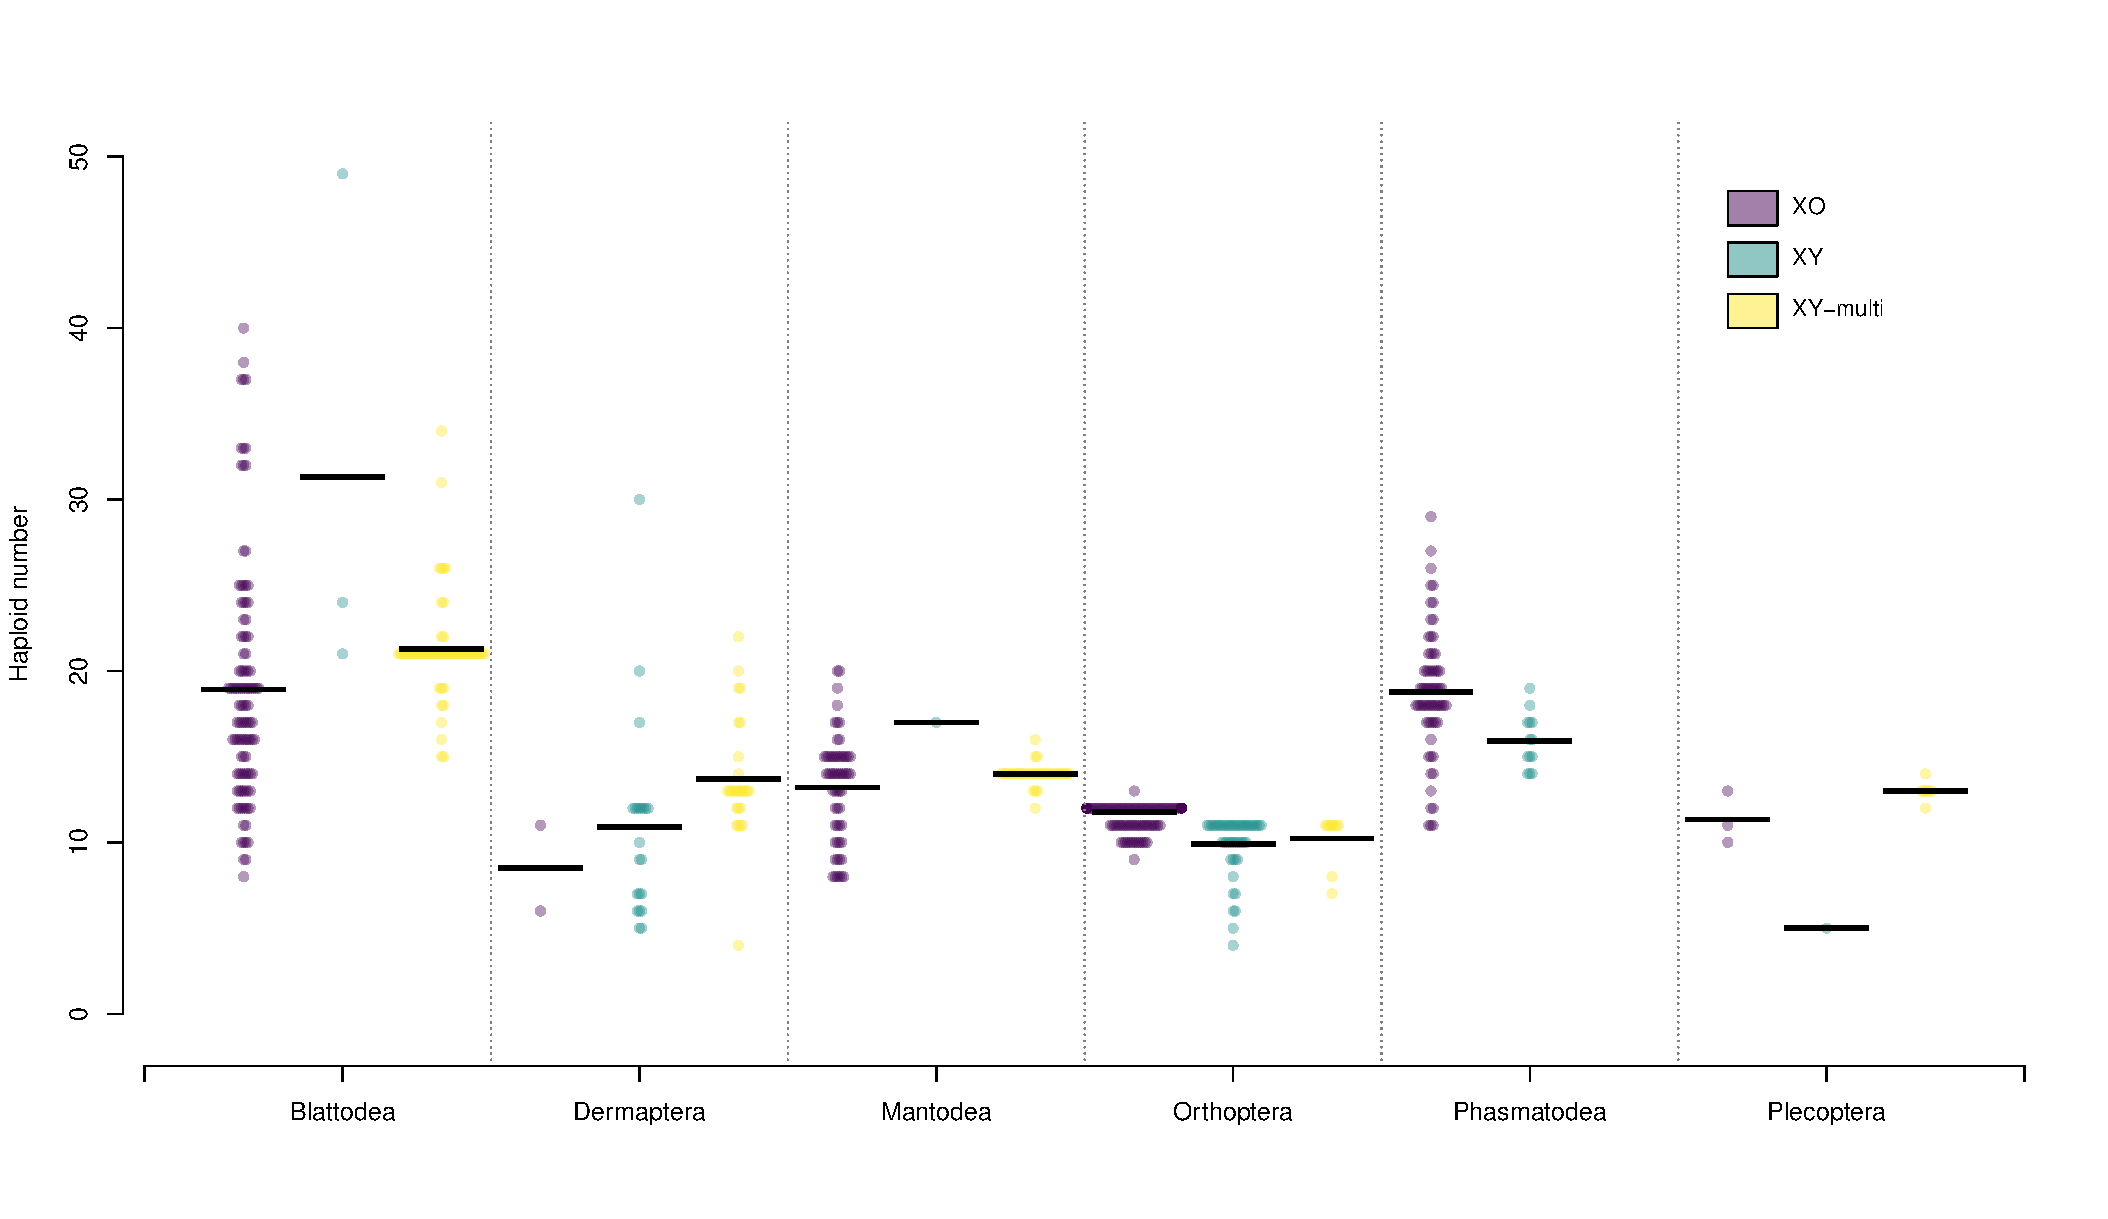
\includegraphics[width=.7\textwidth]{figures/Preliminary_data.pdf}
\caption{
Variation in chromosome numbers with respect to the sex chromosome system in six Polyneoptera orders. Vertical axis indicates the haploid chromosome count. dashed lines represent standard error of the mean.
}
\label{fig:order.plots}
\end{figure}

\newpage
\begin{figure}[h]
\centering 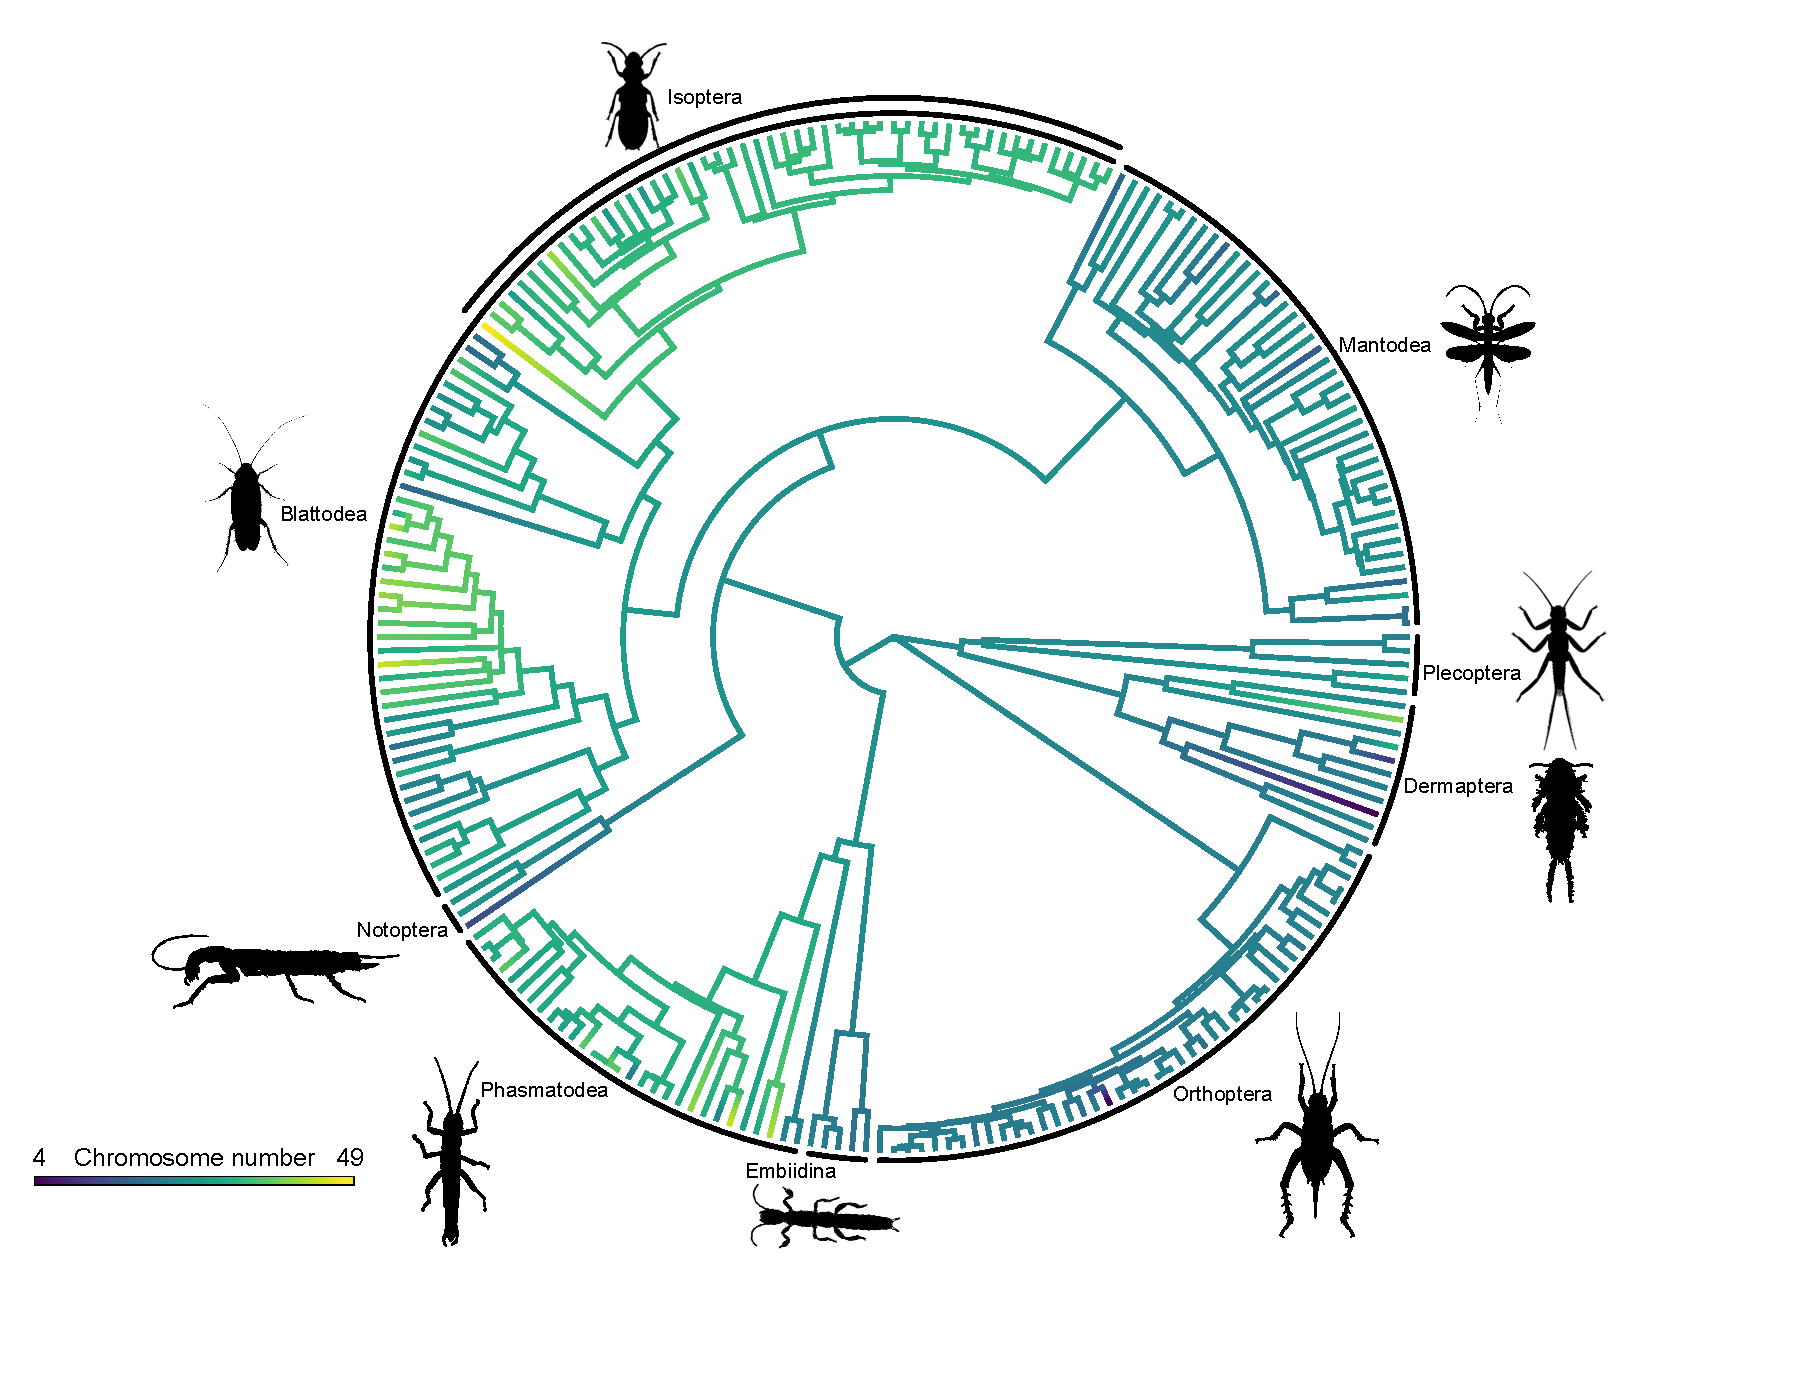
\includegraphics[width=1\textwidth]{figures/phylogenetic_tree.pdf}
\caption{
One of the 100 posterior distribution of trees giving a visual representation of the phylogenetic relationship of the orders in the Polyneoptera clade. The solid black line indicates the taxa for that perticular order. Isoptera is included within Blattodea as it has been identified as a highly derived clade within Blattodea. Branches are coloured according to the chromosome number of that lineage. 
}
\label{fig:phyloplot}
\end{figure}

\newpage
\begin{figure}[h]
\centering 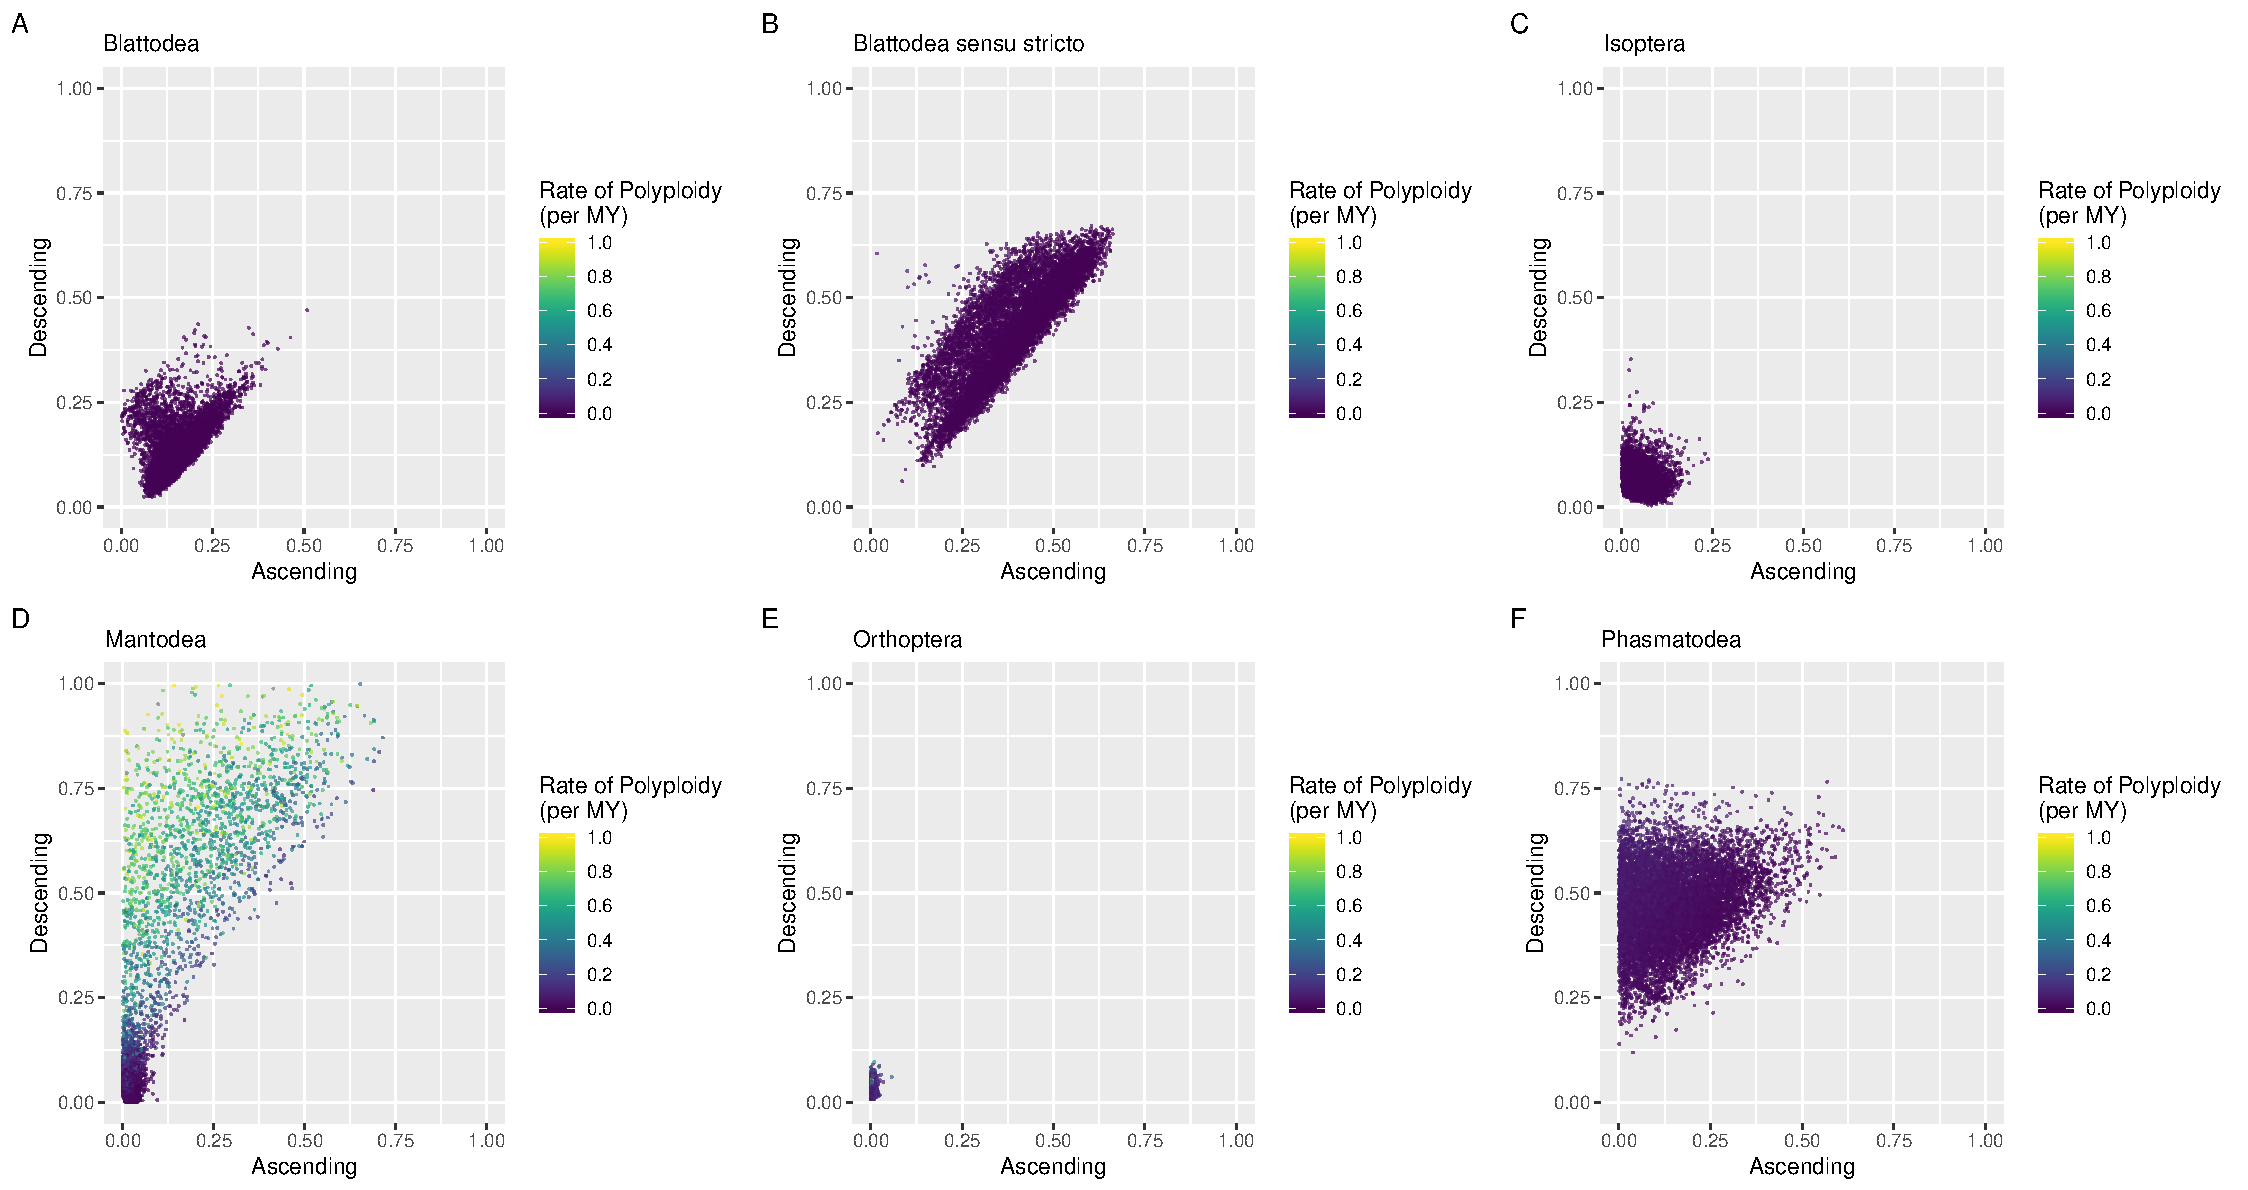
\includegraphics[width=1\textwidth]{figures/rate_distributions_fixed_scale.pdf}
\caption{
Rates of chromosome fission (ascending) and fusion (descending) in five orders of Polyneoptera. Here these rates are color coded according to the rate of polyploidy in each order. 
}
\label{fig:rates}
\end{figure}

\newpage
\begin{figure}[ht]
\centering 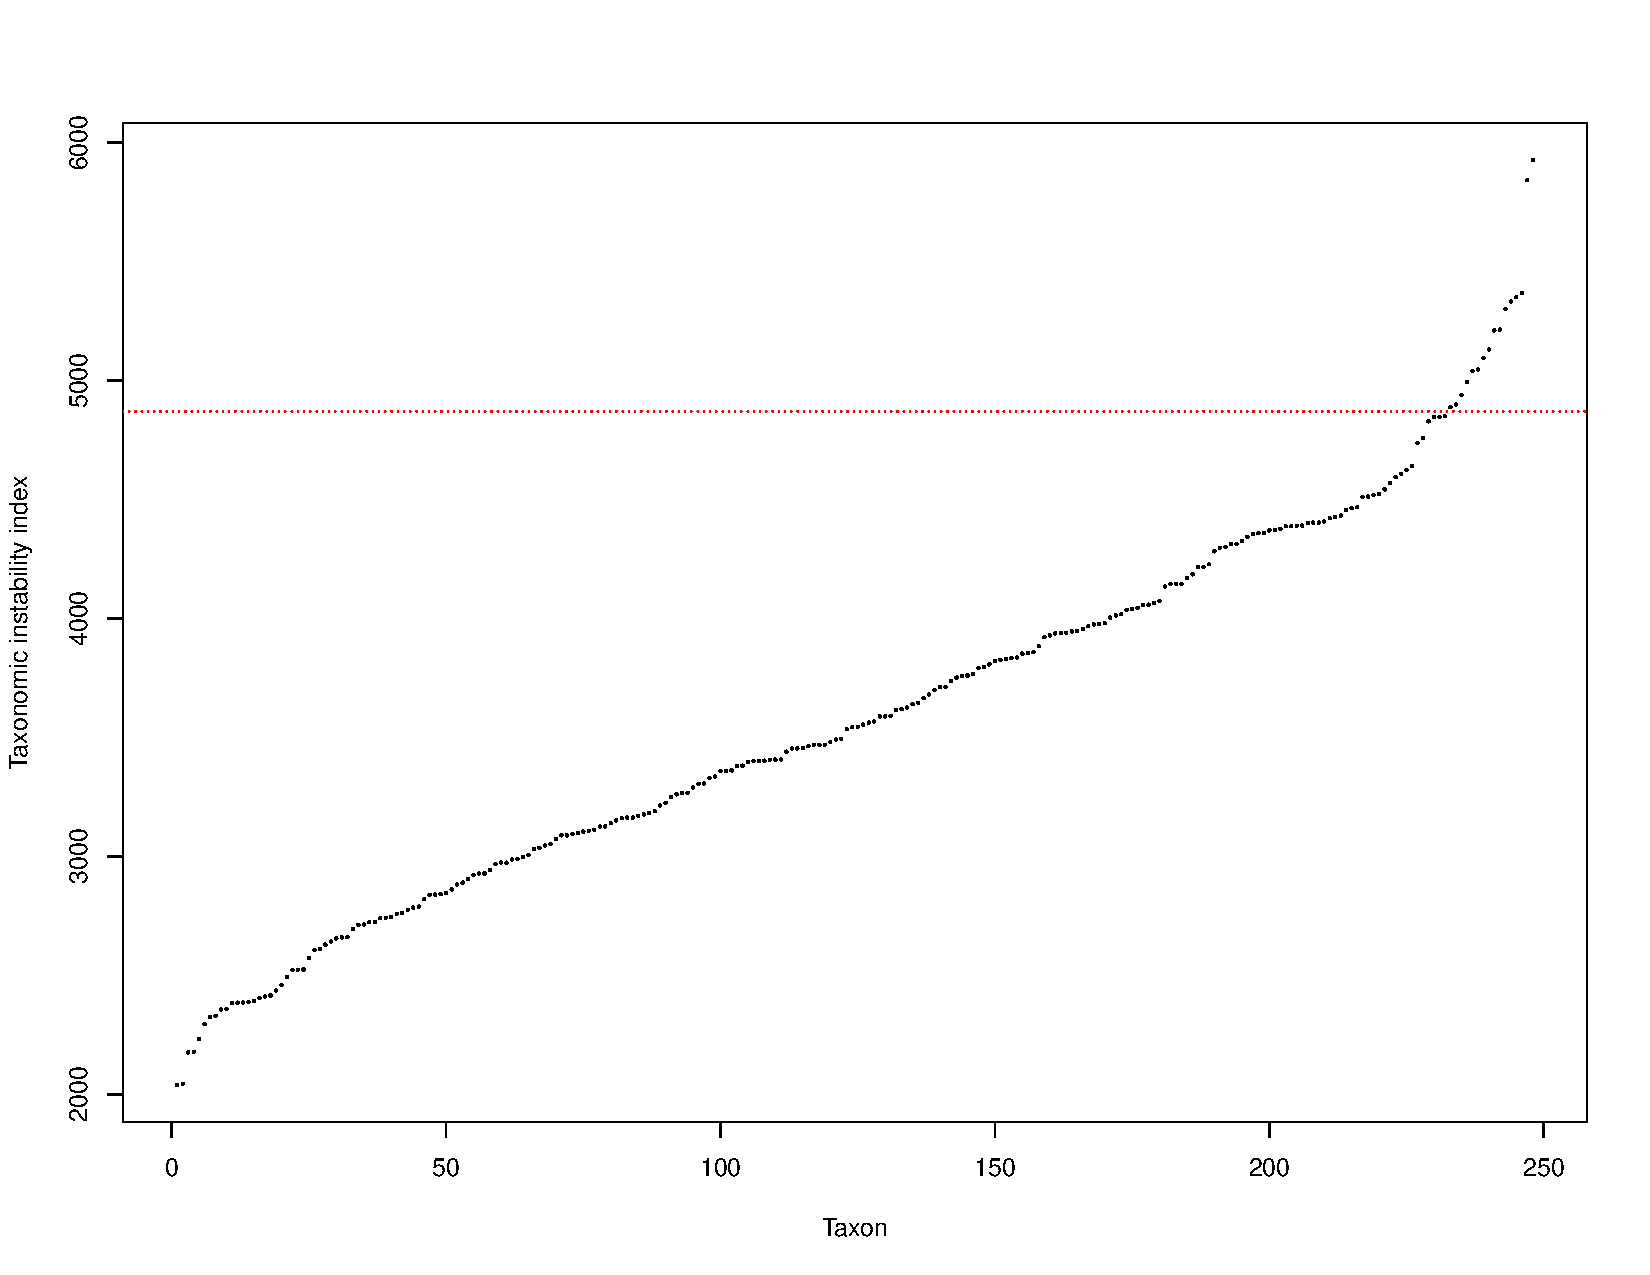
\includegraphics[width=.5\textwidth]{figures/taxonomic_instability_index_plot.pdf}
\caption{
Red dotted line represents the cutoff point of 4780. Roughly about 94\% of the taxa fall below this cutoff point
}
\label{fig:tax.index}
\end{figure}

\newpage
\begin{figure}
\centering 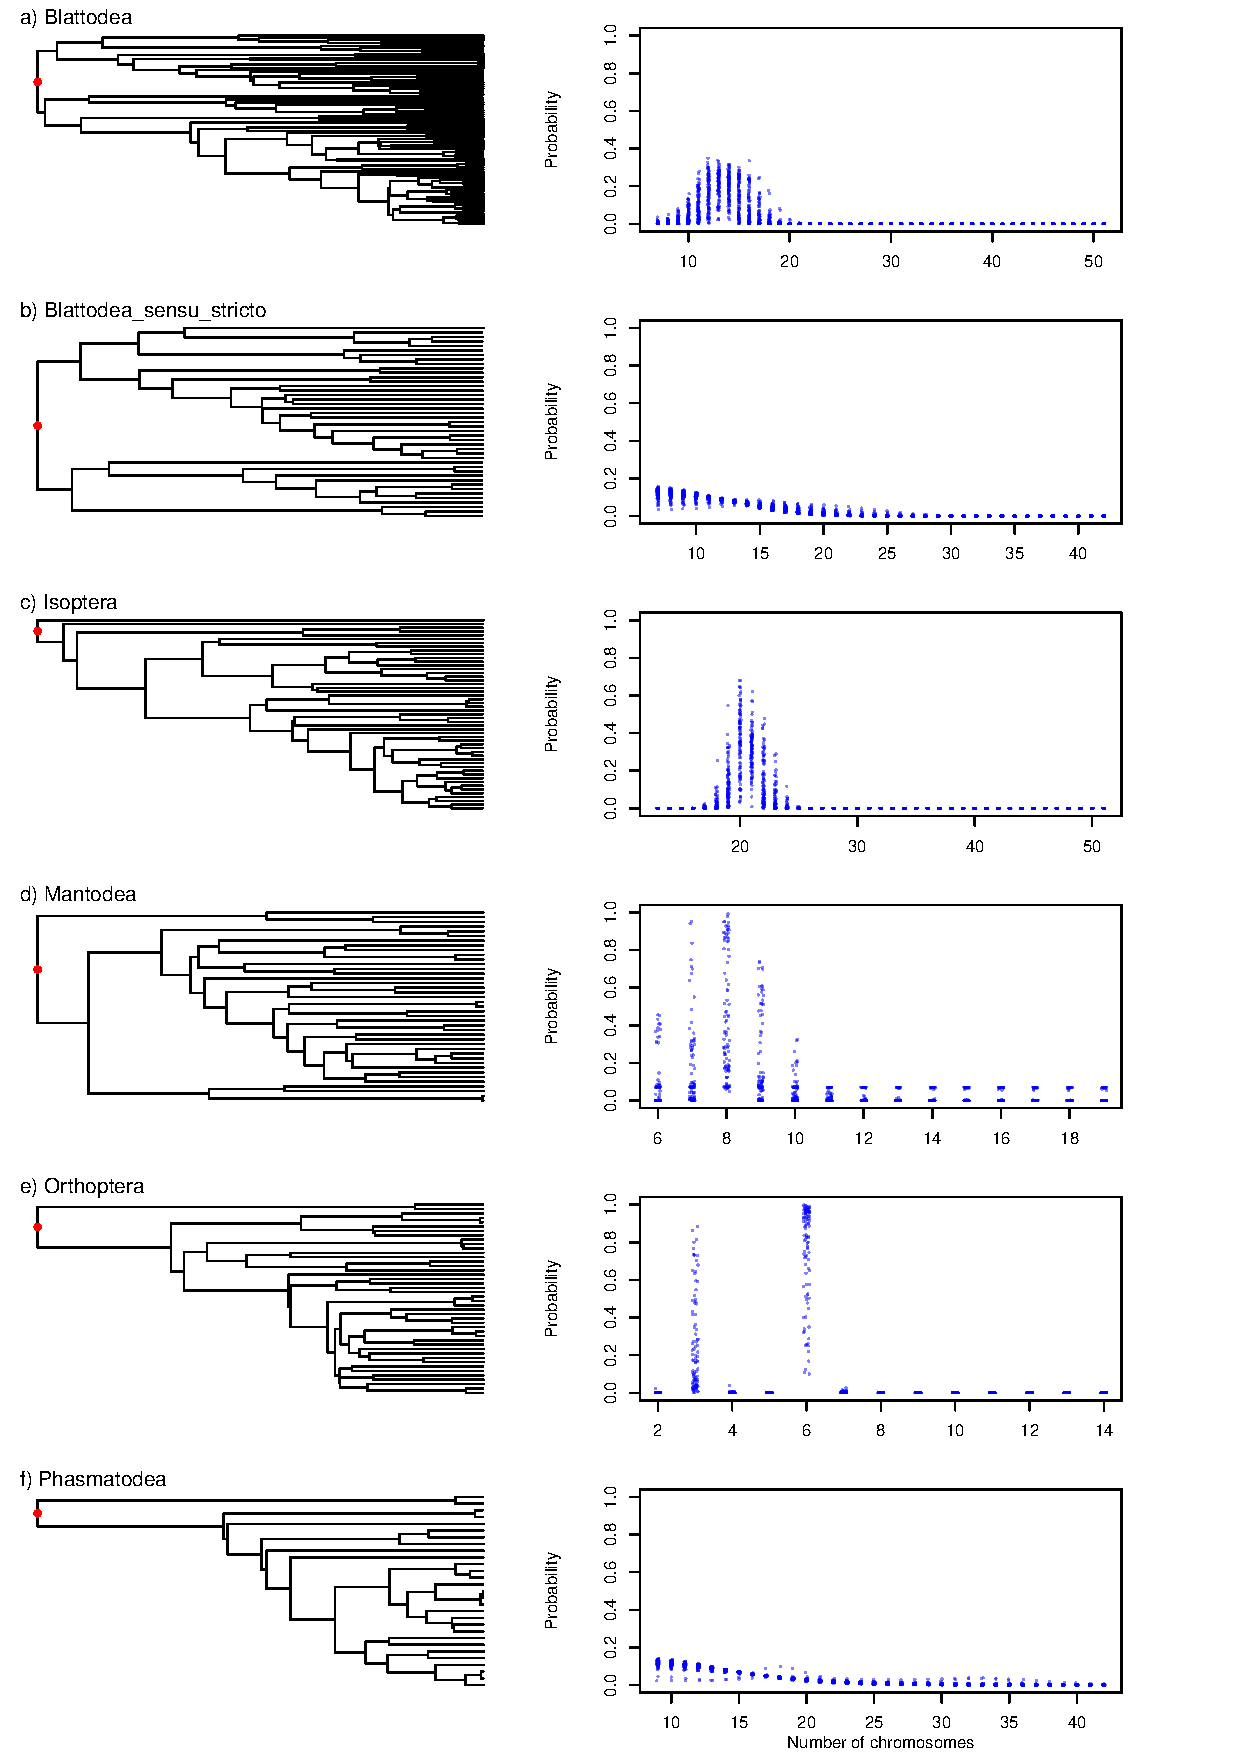
\includegraphics[width=.7\textwidth]{figures/asr_plot.pdf}
\caption{Ancestral states reconstruction of the studied taxa. The root of each clade is indicated by red dot. Except for Orthoptera where we see chromosome numbers three and six as the only inferred ancestral states, we find a normal distribution for ancestral states in all other clades.}
\label{fig:asr}
\end{figure}

\newpage
\begin{figure}
\centering 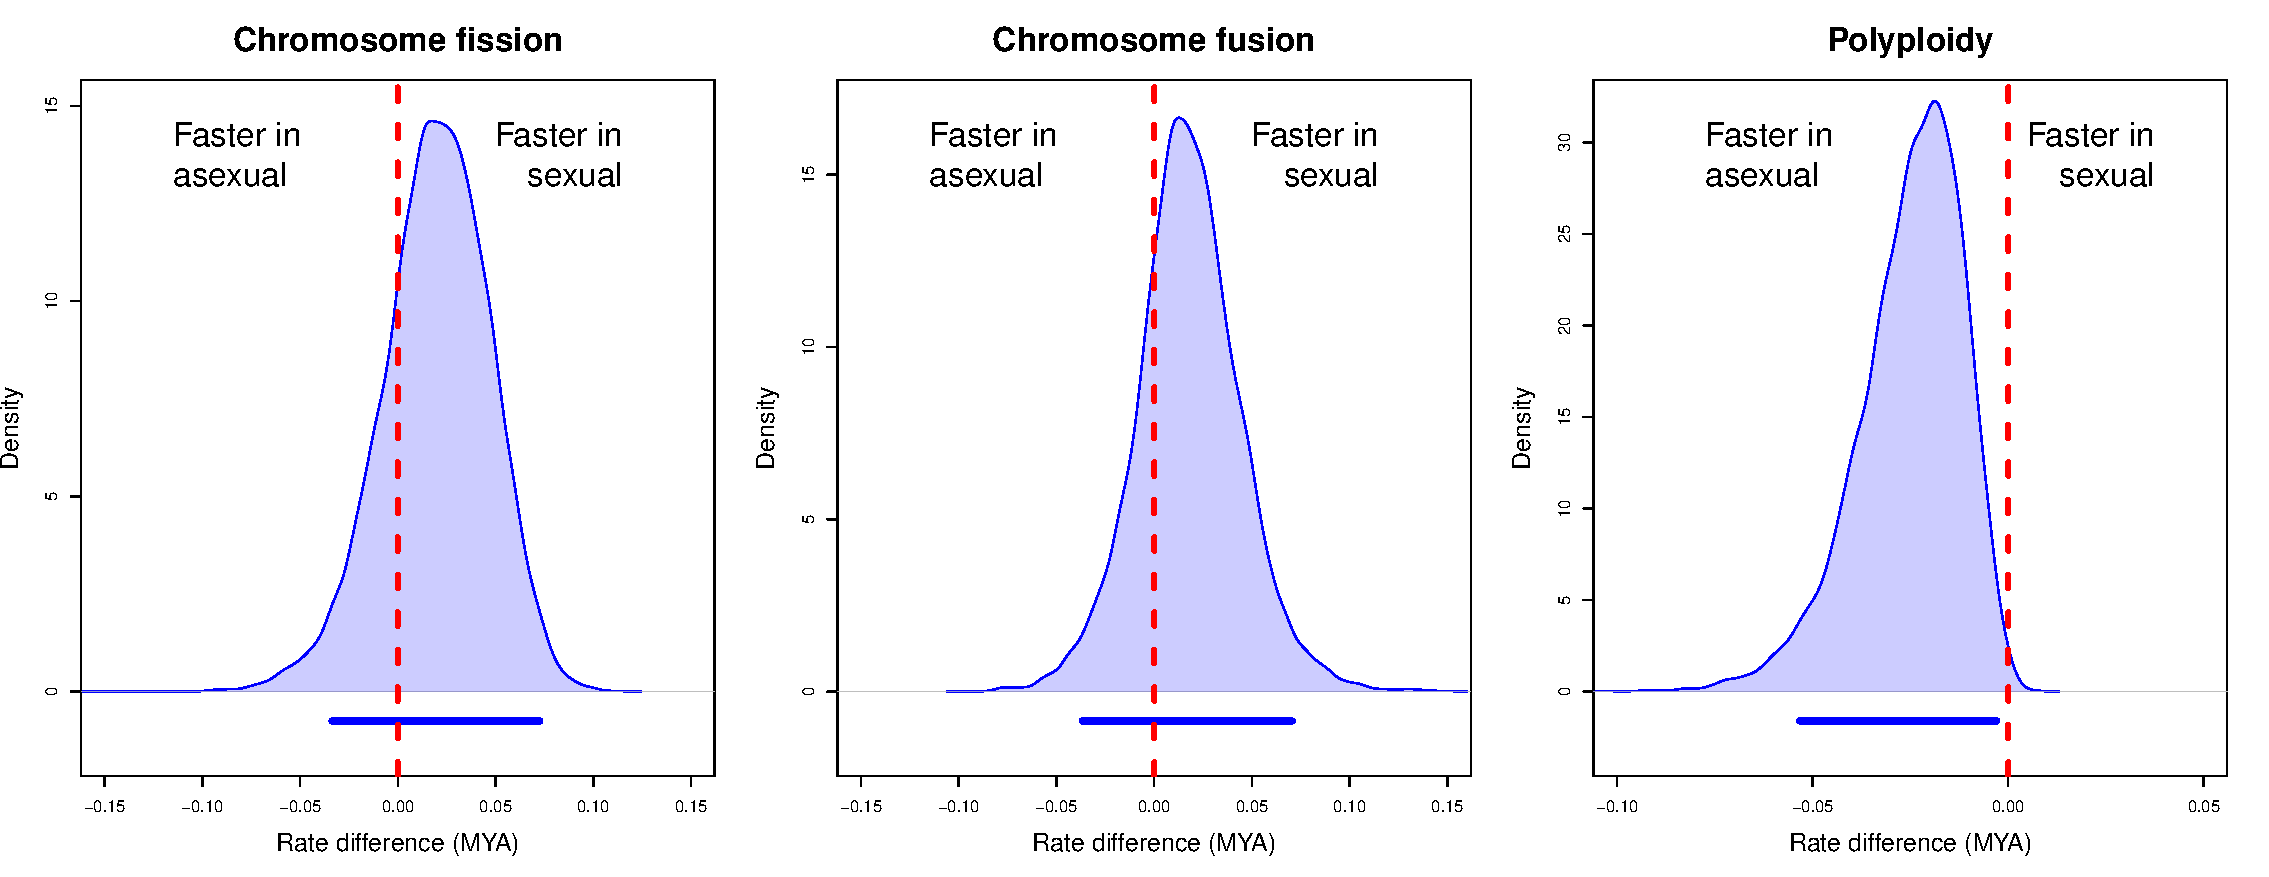
\includegraphics[width=.7\textwidth]{figures/phasmatodea_sex_asex_plot.pdf}
\caption{Chromosome evolution rates in sexual and asexual reproducing systems in the order Phasmatodea. Bars below the plot indicates the 95\% HPD interval}
\label{fig:phas.plot}
\end{figure}

\newpage
\begin{figure}
\centering 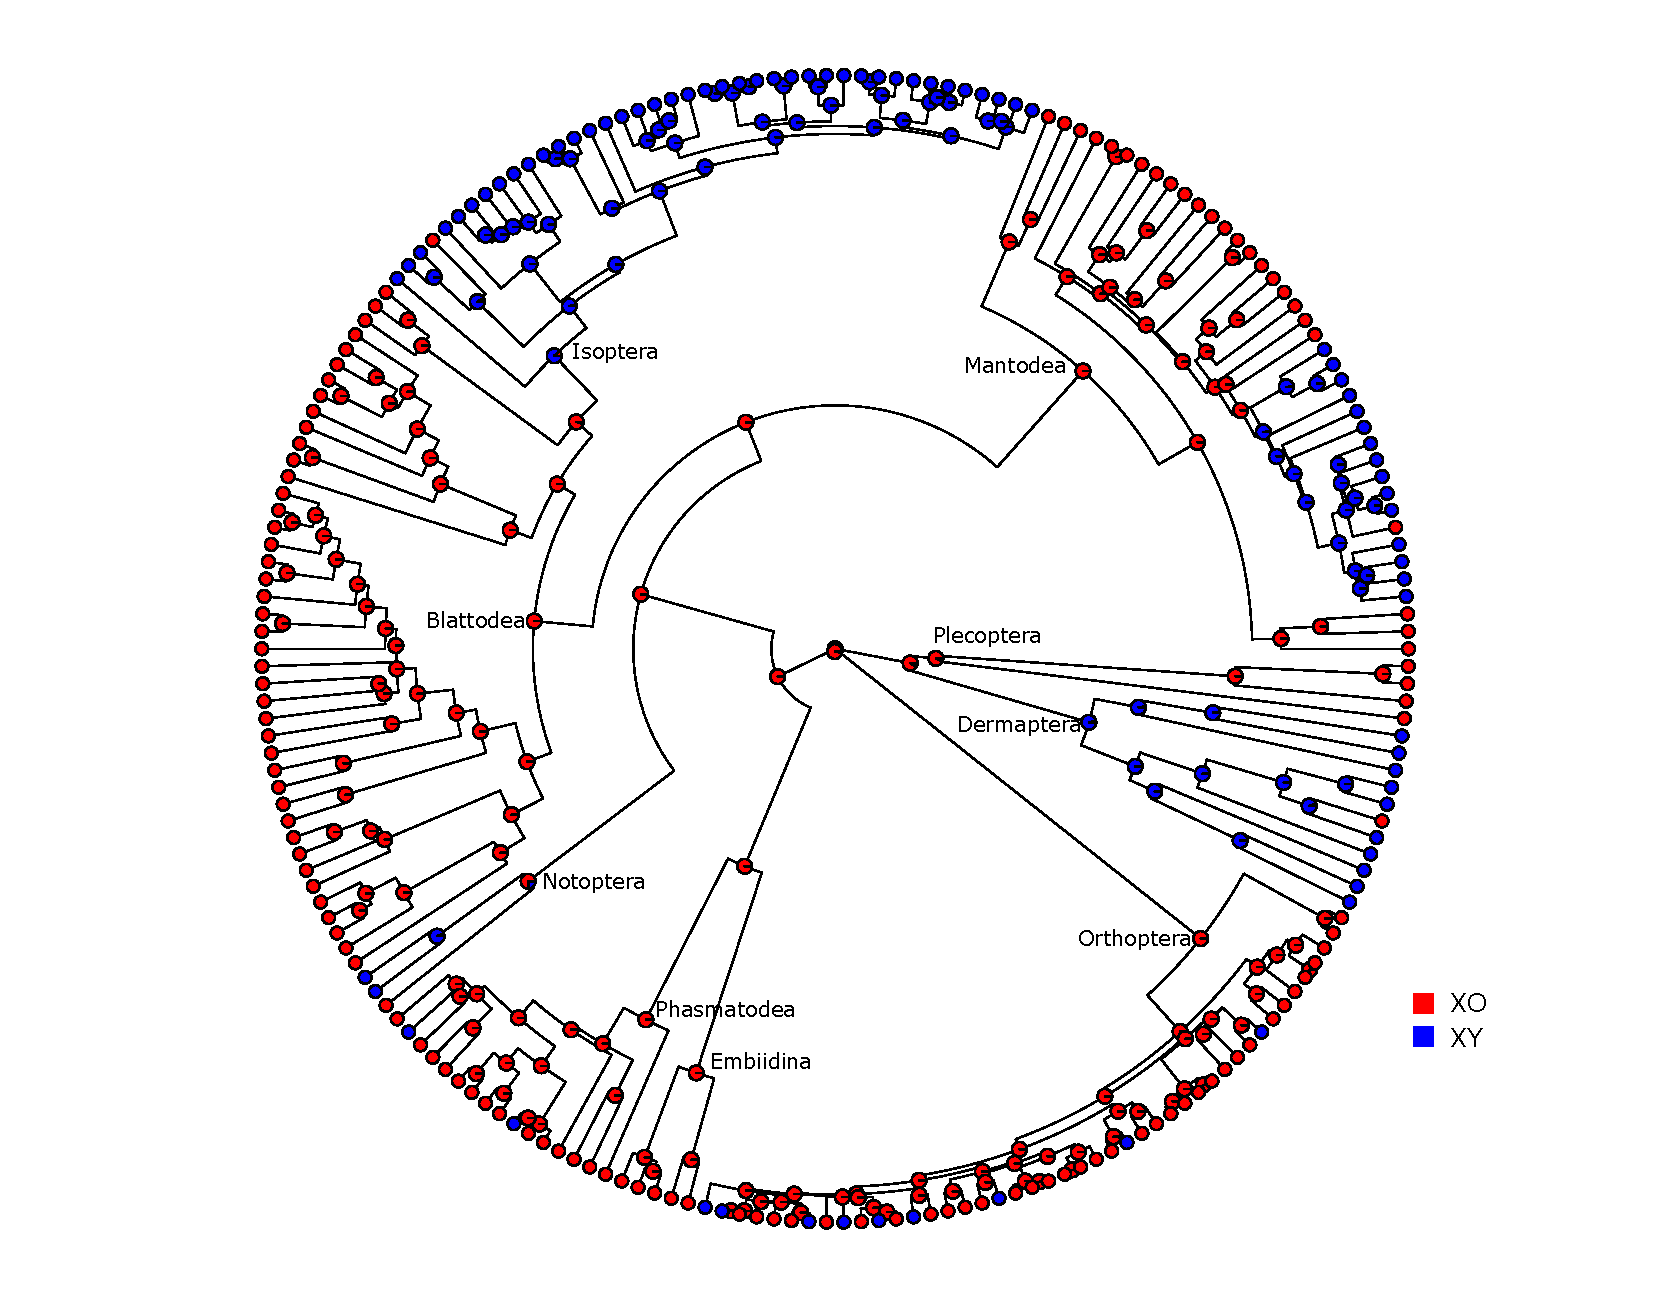
\includegraphics[width=1\textwidth]{figures/sex_chrom_asr_phylogeny.pdf}
\caption{Ancestral states reconstruction of the sex chromosome systems. This is a single tree of the posterior distribution. Red colour represents XO sex chromosome system and Blue colour represents XY sex chromosome systems. Order names are marked at the origin of each order. The probabilities of each sex chromosome system as being the ancestral state is given by the respective coloured potion of the pi charts at each node. Tip colours represent the current state of the sex chromosome system.}
\label{fig:sex.asr.plot}
\end{figure}

\newpage
\begin{figure}
\centering 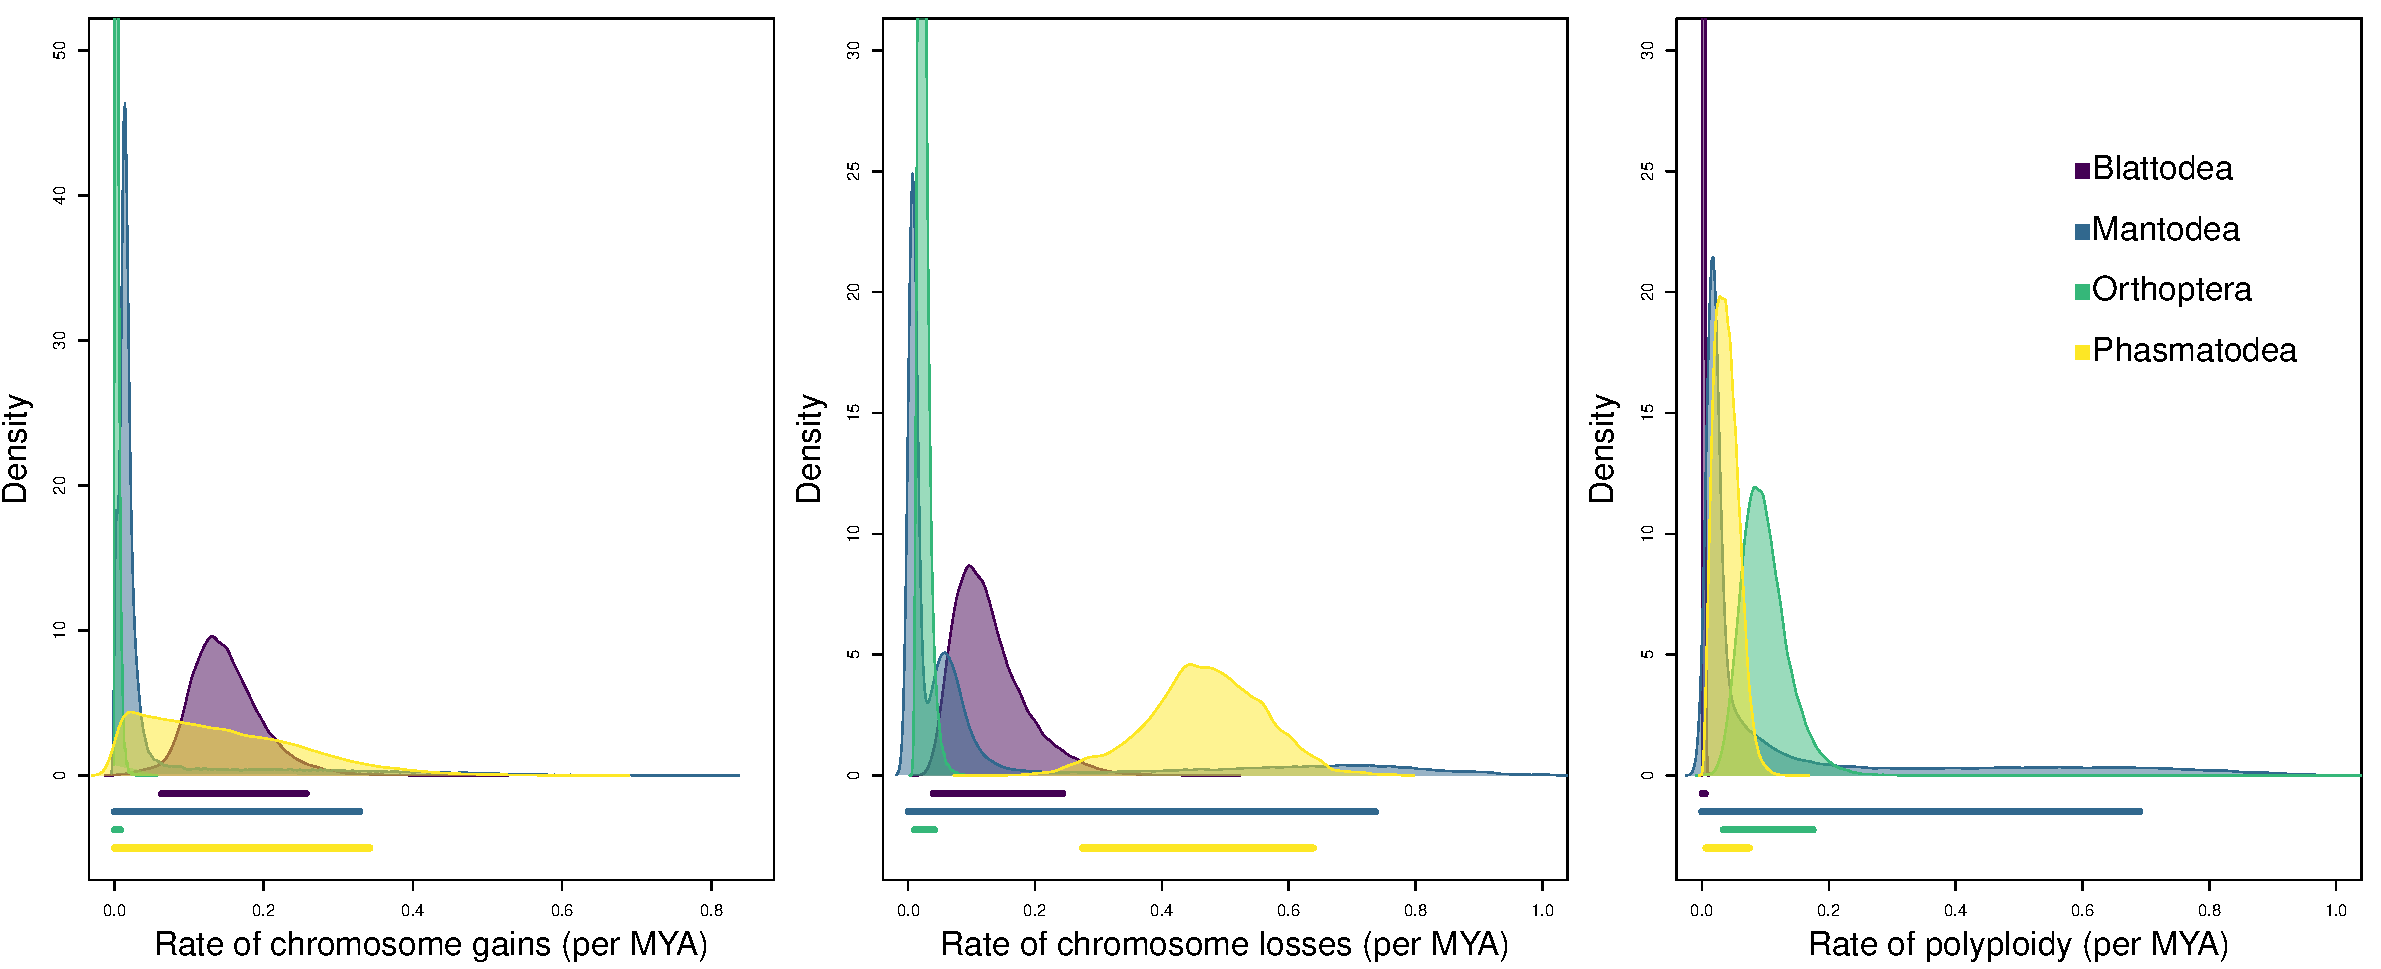
\includegraphics[width=.7\textwidth]{figures/order_rates_95HPD.pdf}
\caption{Rates of chromosome fusion, fission and, polyploidy of four orders in the insect clade Phasmatodea. The y axis is shortened to show the spread of these rates. The bars below each distribution indicates the 95\% HPD interval}
\label{fig:order.rates.95HPD}
\end{figure}


\begin{table}
\centering
\begin{tabular}{llccccc}
\hline
\multirow{2}{*}{Order} & \multirow{2}{*}{Genus} & \multicolumn{3}{l}{\begin{tabular}[c]{@{}c@{}}Mean number of\\ chromosomes\end{tabular}} & \multicolumn{2}{l}{Evidence supports} \\ \cline{3-7} 
                       &                        & XO                          & XY                          & multi                        & Fusion            & Fission           \\ \hline
Orthoptera             & Aleuas                 & 10                          & 10.2                        & -                            & -                 & -                 \\
Orthoptera             & Dichroplus             & 11.7                        & 9.7                         & 11                           & +                 & +                 \\
Orthoptera             & Diponthus              & 11.5                        & 11                          & -                            & +                 & -                 \\
Orthoptera             & Eurotettix             & -                           & 11                          & 11                           & -                 & -                 \\
Orthoptera             & Gryllotalpa            & 10.7                        & 6                           & -                            & +                 & -                 \\
Orthoptera             & Leiotettix             & 12                          & 9                           & 7.5                          & +                 & -                 \\
Orthoptera             & Scotussa               & 11.6                        & 9.5                         & 11                           & +                 & +                 \\
Orthoptera             & Scyllina               & 12                          & 11                          & -                            & +                 & -                 \\
Orthoptera             & Tetrixocephalus        & 12                          & 11                          & -                            & +                 & -                 \\
Orthoptera             & Xyleus                 & 12                          & 11                          & -                            & +                 & -                 \\
Orthoptera             & Zoniopoda              & 12                          & 11                          & -                            & +                 & -                 \\
Phasmatodea            & Didymuria              & 18.6                        & 15.4                        & -                            & +                 & -                 \\
Phasmatodea            & Isagoras               & 19                          & 17                          & -                            & +                 & -                 \\
Phasmatodea            & Leptynia               & 19.2                        & 18                          & -                            & +                 & -                 \\
Phasmatodea            & Podacanthus            & 18                          & 14                          & -                            & +                 & -                 \\
Phasmatodea            & Prisopus               & 25                          & 14                          & -                            & +                 & -                 \\
Mantodea               & Deiphobe               & 10                          & -                           & 14                           & -                 & -                 \\
Dermaptera             & Forficula              & -                           & 12                          & 12.8                         & -                 & +                 \\
Dermaptera             & Nala                   & -                           & 18.5                        & 19                           & -                 & +                 \\
Dermaptera             & Nesogaster             & 11                          & -                           & 11                           & -                 & -                 \\
Plecoptera             & Perla                  & 10.5                        & 5                           & 12.8                         & +                 & +                 \\ \hline
\end{tabular}
\caption{Chromsome number and sex chromosome systems. In each genus we report the mean number of chromosomes for all species having each type of sex chromosome systems. The fusion and fission columns contain a + to indicate a difference of chromosome number that is consistent with either fusions or fissions. A - symbol indicates a distribution of chromosome number that is uninformative.}
\label{tab:fusions}
\end{table}

\begin{table}[ht]
\centering
\begin{tabular}{lccc}
\hline
\textbf{Order}          & \textbf{Fission} & \textbf{Fusion} & \textbf{Polyploidy} \\ \hline
Blattodea               & 0.063 - 0.257    & 0.040 - 0.243    & 0.000 - 0.005           \\
Blattodea sensu stricto & 0.173 - 0.604    & 0.202 - 0.619   & 0.000 - 0.010            \\
Isoptera                & 0.002 - 0.100      & 0.019 - 0.114   & 0.000 - 0.006           \\
Mantodea                & 0.000 - 0.329        & 0.000 - 0.737       & 0.000 - 0.69            \\
Orthoptera              & 0.000 - 0.008        & 0.010 - 0.041    & 0.034 - 0.175       \\
Phasmatodea             & 0.000 - 0.342        & 0.275 - 0.639   & 0.006 - 0.074       \\ \hline
\end{tabular}
\caption{95\% Highest posterior density distribution for chromosome fissions, fusions and polyploidy of the four orders}
\label{tab:HPD}
\end{table}
\clearpage
\section{Supplemental}
\vfill

\setcounter{figure}{0}
\renewcommand{\thefigure}{S\arabic{figure}}
\setcounter{table}{0}
\renewcommand{\thetable}{S\arabic{table}}

\begin{figure}[!ht]
\centering 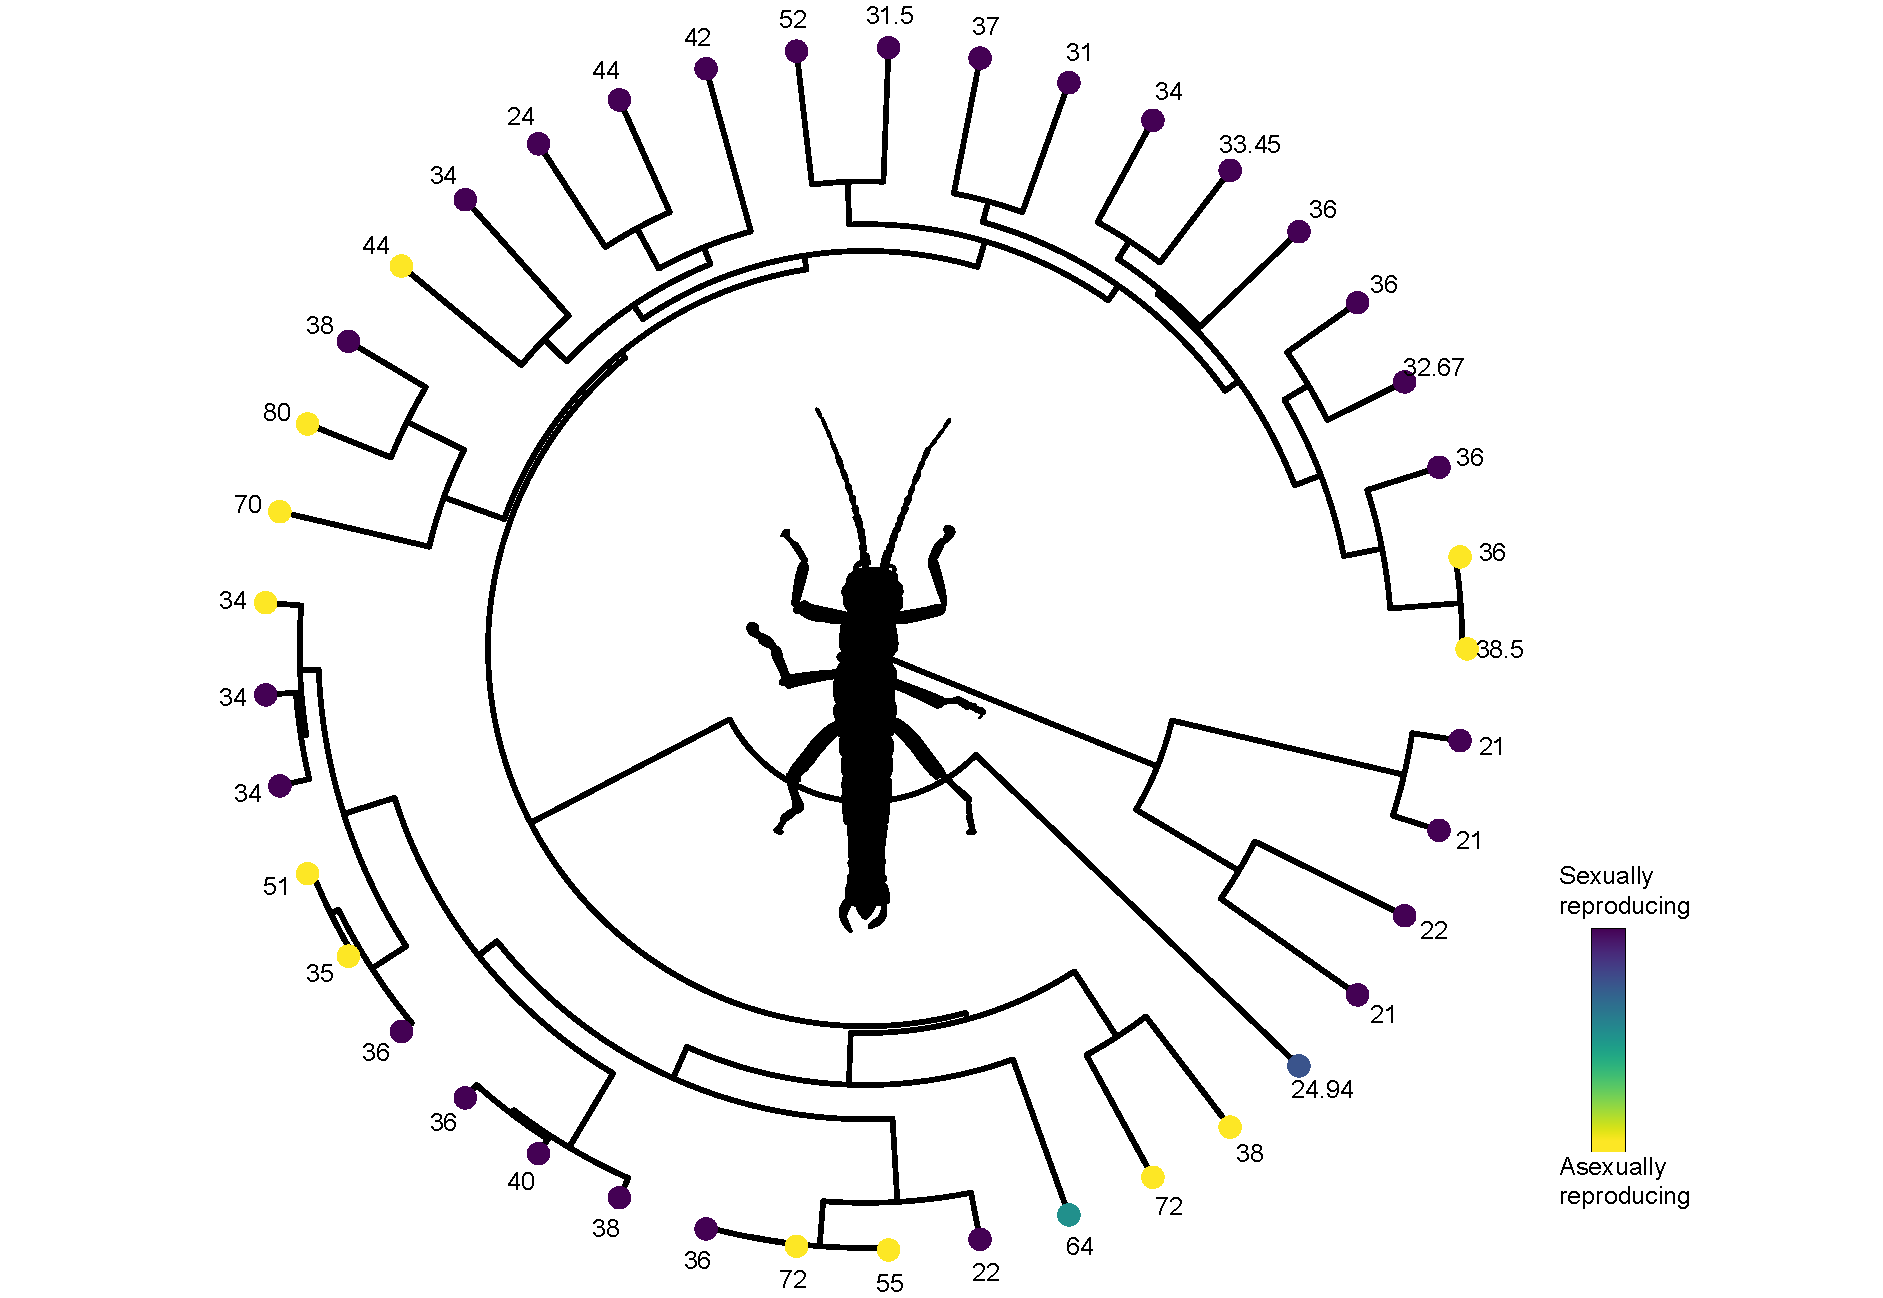
\includegraphics[width=1\textwidth]{figures/phasmatodea_phylogeny.pdf}
\caption{Phylogeny of the insect clade Phasmatodea. Tips are colored according to the mode of reproduction (sexual or asexual). Some lineages show intermediate colours. These are lineages which have both sexual and asexual populations. The shade of colour indicates the probability of observig either reproductive modes in these lineages. The numbers indicate the mean chromosome number for each lineage.}
\label{fig:phas.phylo}
\end{figure}

\begin{figure}
\centering 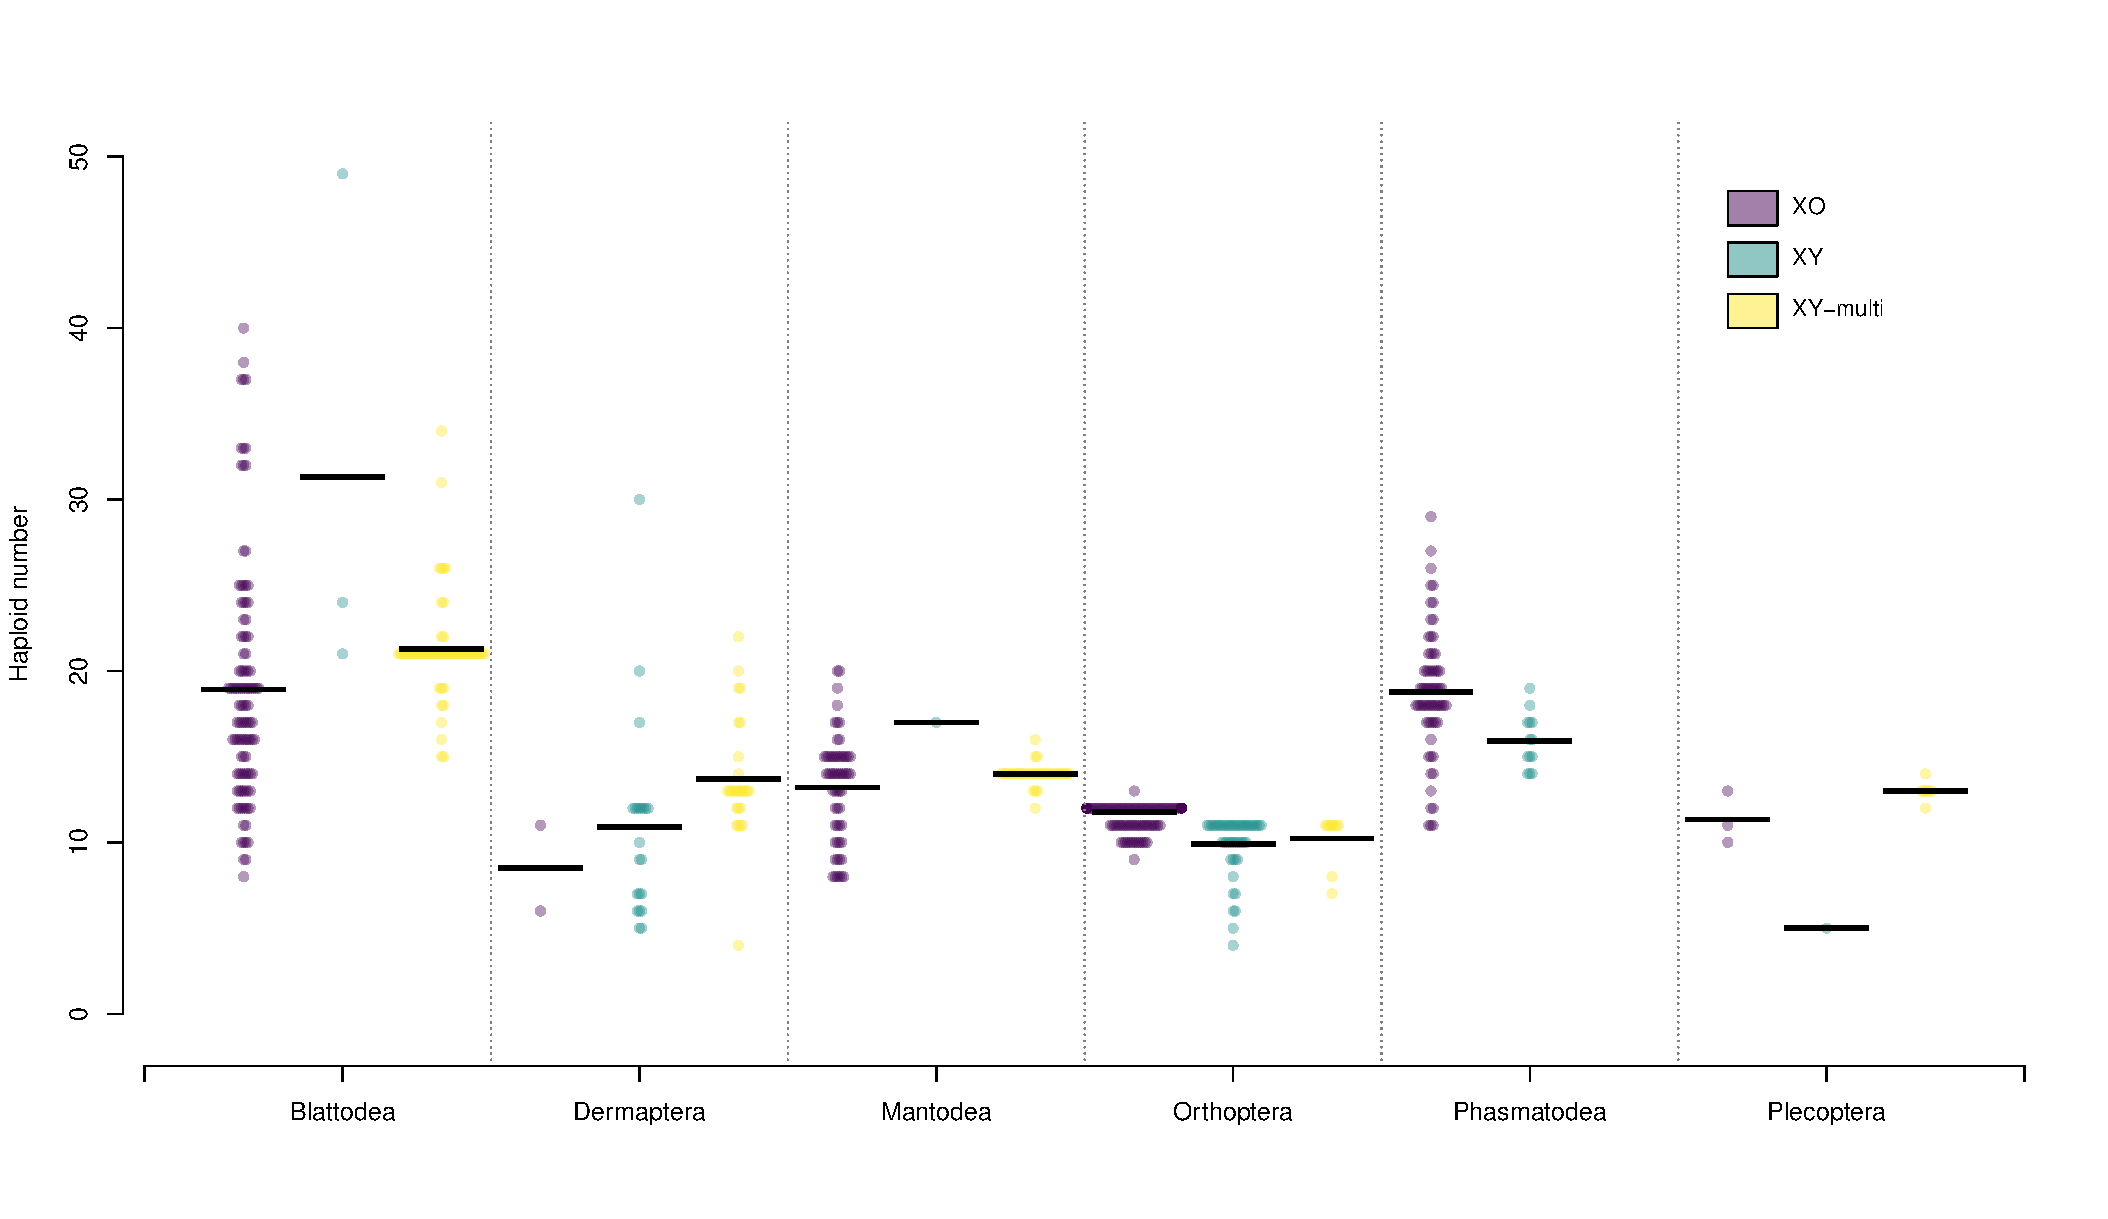
\includegraphics[width=.7\textwidth]{figures/Preliminary_data.pdf}
\caption{
Variation in chromosome numbers with respect to the sex chromosome system in six Polyneoptera orders. Vertical axis indicates the haploid chromosome count. dashed lines represent standard error of the mean.
}
\label{fig:order.plots}
\end{figure}

\begin{figure}
\centering 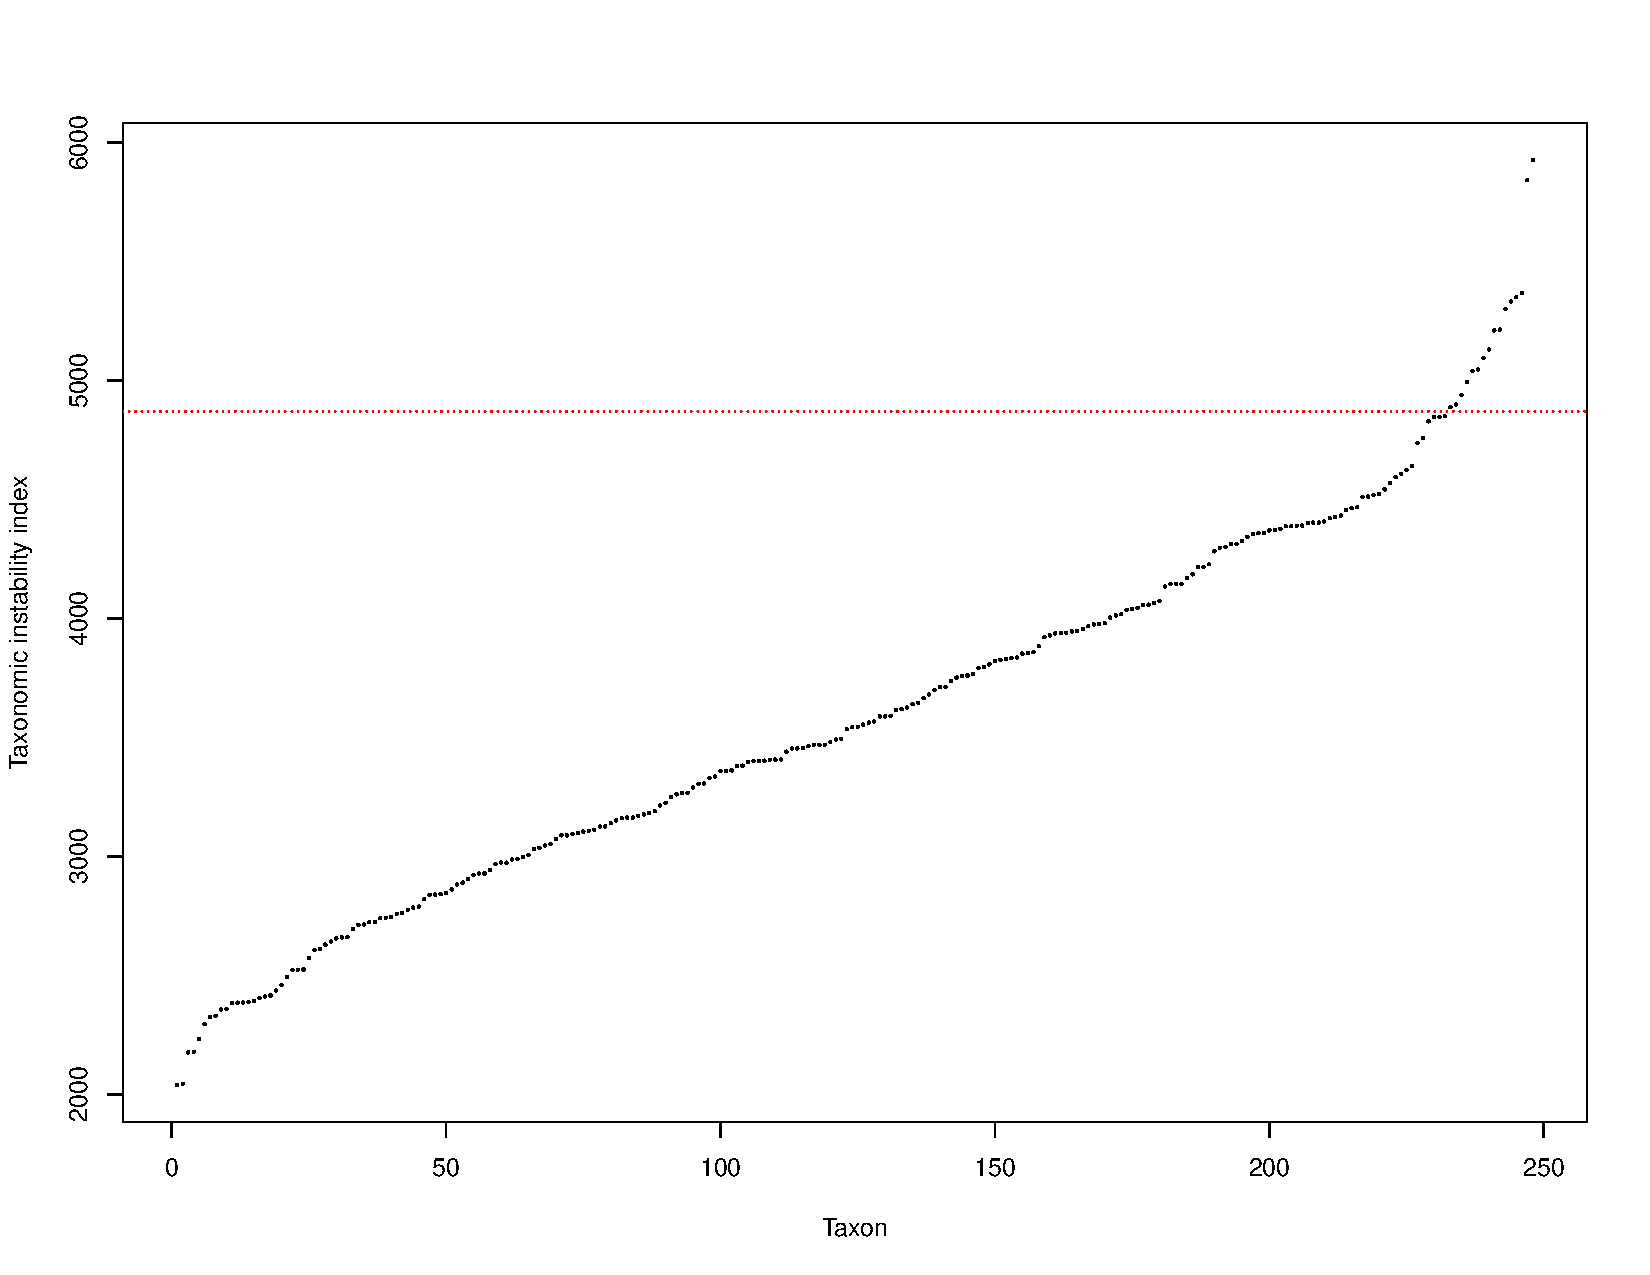
\includegraphics[width=.5\textwidth]{figures/taxonomic_instability_index_plot.pdf}
\caption{
Red dotted line represents the cutoff point of 4780. Roughly about 94\% of the taxa fall below this cutoff point
}
\label{fig:tax.index}
\end{figure}

\begin{figure}
\centering 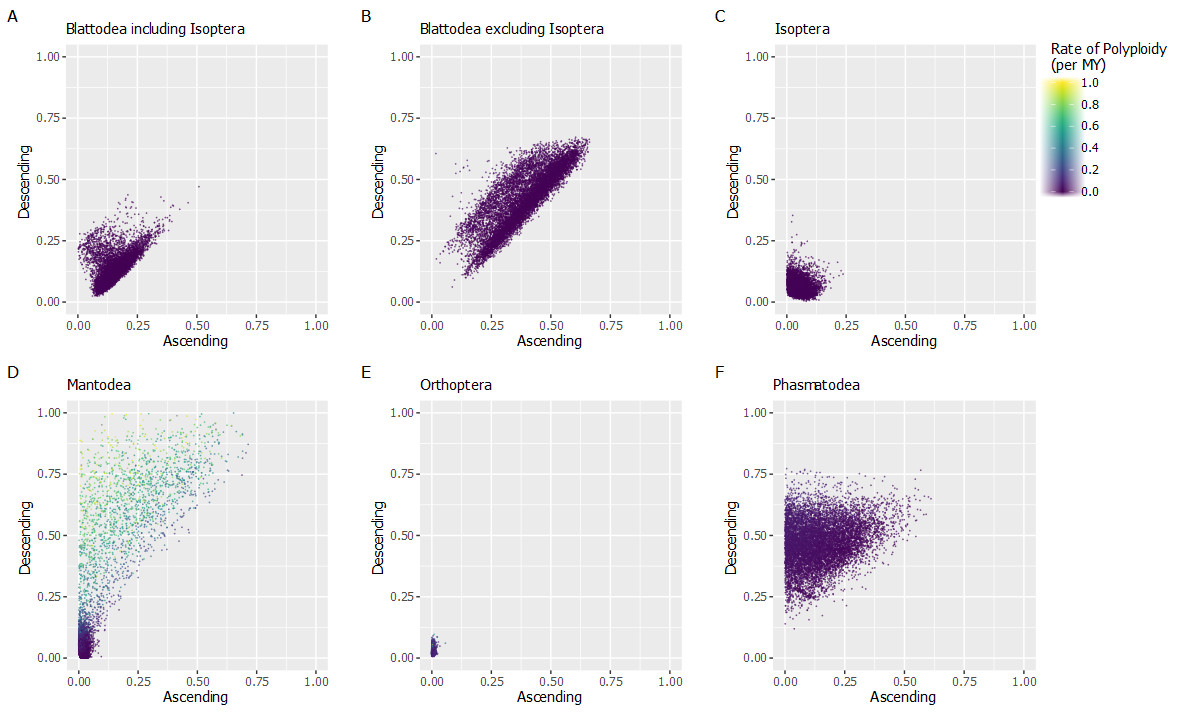
\includegraphics[width=1\textwidth]{figures/rate_estimates.jpg}
\caption{
Rates of chromosome fission (ascending) and fusion (descending) in five orders of Polyneoptera. Here these rates are color coded according to the rate of polyploidy in each order. 
}
\label{fig:rates}
\end{figure}

\begin{figure}
\centering 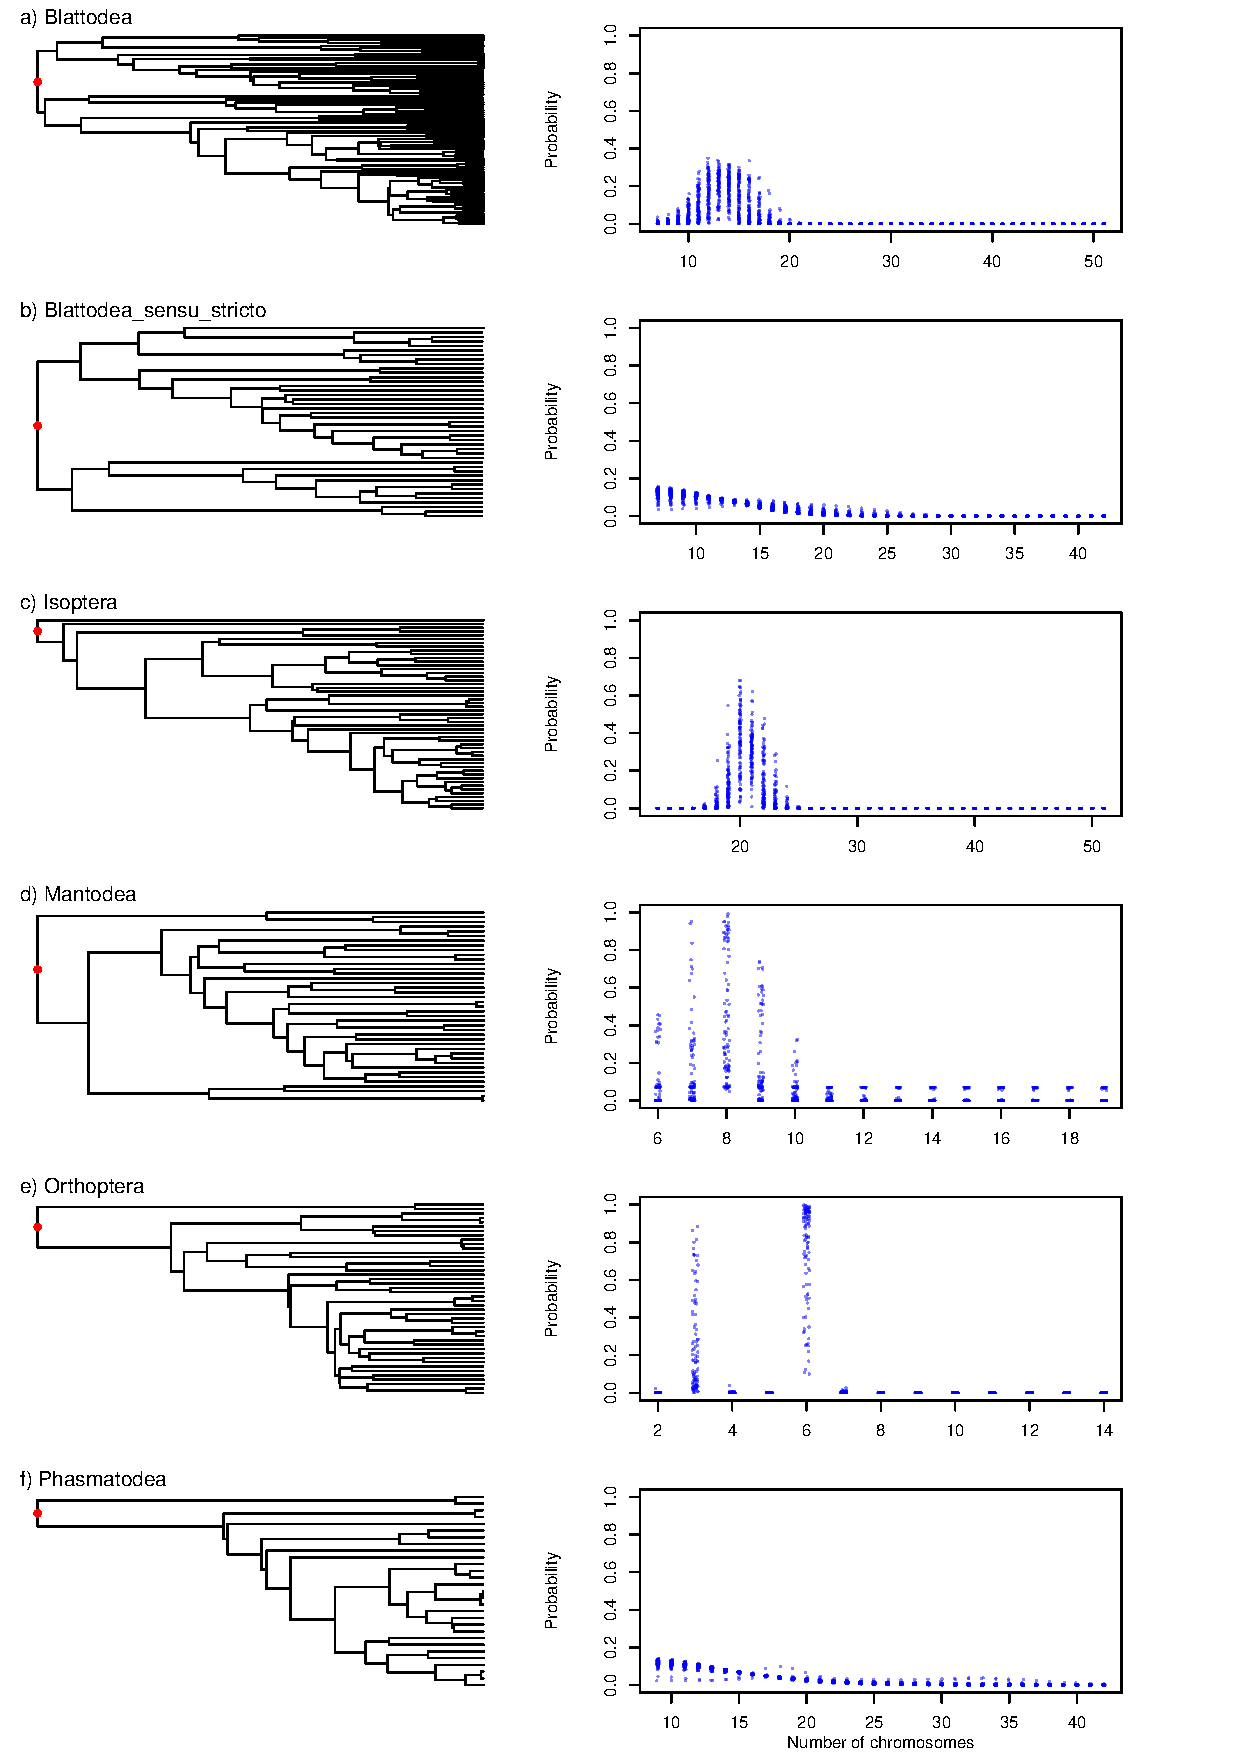
\includegraphics[width=.7\textwidth]{figures/asr_plot.pdf}
\caption{Ancestral states reconstruction of the studied taxa. The root of each clade is indicated by red dot. Except for Orthoptera where we see chromosome numbers three and six as the only inferred ancestral states, we find a normal distribution for ancestral states in all other clades.}
\label{fig:asr}
\end{figure}

\begin{table}[ht]
\begin{tabular}{lcc}
\hline
\textbf{Transition} & \textbf{Mean rate (95\% credible interval)} & \textbf{Mean number of transitions} \\ \hline
XO to XY            & 0.0020 (0.0015 - 0.0026)                    & 15.3                                \\
XY to XO            & 0.0021 (0.0010 - 0.0036)                    & 6.7                                 \\ \hline
\end{tabular}
\caption{Mean transition rates and mean number of transitions obtained from stochastic mapping of sex chromosome transitions}
\label{tab:simmap.summary}
\end{table}

\begin{table}
\centering
\begin{tabular}{ll}
\hline
\textbf{Mean rate (95\% Credible Interval)}  & \textbf{Mean number of transitions} \\ \hline
\multicolumn{1}{c}{0.0063 (0.0052 - 0.0078)} & \multicolumn{1}{c}{9.3}             \\ \hline
\end{tabular}
\caption{Mean rate of transition from sexual reproduction to parthenogenesis and mean number of 
such transitions estimated from stochastic mapping. The transition rate of parthenogenesis to sexual reproducing was set to zero}
\label{tab:phas.simmap.summary}
\end{table}


\end{document}
